% Options for packages loaded elsewhere
\PassOptionsToPackage{unicode}{hyperref}
\PassOptionsToPackage{hyphens}{url}
%
\documentclass[
  english,
  man]{apa6}
\usepackage{amsmath,amssymb}
\usepackage{lmodern}
\usepackage{ifxetex,ifluatex}
\ifnum 0\ifxetex 1\fi\ifluatex 1\fi=0 % if pdftex
  \usepackage[T1]{fontenc}
  \usepackage[utf8]{inputenc}
  \usepackage{textcomp} % provide euro and other symbols
\else % if luatex or xetex
  \usepackage{unicode-math}
  \defaultfontfeatures{Scale=MatchLowercase}
  \defaultfontfeatures[\rmfamily]{Ligatures=TeX,Scale=1}
\fi
% Use upquote if available, for straight quotes in verbatim environments
\IfFileExists{upquote.sty}{\usepackage{upquote}}{}
\IfFileExists{microtype.sty}{% use microtype if available
  \usepackage[]{microtype}
  \UseMicrotypeSet[protrusion]{basicmath} % disable protrusion for tt fonts
}{}
\makeatletter
\@ifundefined{KOMAClassName}{% if non-KOMA class
  \IfFileExists{parskip.sty}{%
    \usepackage{parskip}
  }{% else
    \setlength{\parindent}{0pt}
    \setlength{\parskip}{6pt plus 2pt minus 1pt}}
}{% if KOMA class
  \KOMAoptions{parskip=half}}
\makeatother
\usepackage{xcolor}
\IfFileExists{xurl.sty}{\usepackage{xurl}}{} % add URL line breaks if available
\IfFileExists{bookmark.sty}{\usepackage{bookmark}}{\usepackage{hyperref}}
\hypersetup{
  pdflang={en-EN},
  hidelinks,
  pdfcreator={LaTeX via pandoc}}
\urlstyle{same} % disable monospaced font for URLs
\usepackage{graphicx}
\makeatletter
\def\maxwidth{\ifdim\Gin@nat@width>\linewidth\linewidth\else\Gin@nat@width\fi}
\def\maxheight{\ifdim\Gin@nat@height>\textheight\textheight\else\Gin@nat@height\fi}
\makeatother
% Scale images if necessary, so that they will not overflow the page
% margins by default, and it is still possible to overwrite the defaults
% using explicit options in \includegraphics[width, height, ...]{}
\setkeys{Gin}{width=\maxwidth,height=\maxheight,keepaspectratio}
% Set default figure placement to htbp
\makeatletter
\def\fps@figure{htbp}
\makeatother
\setlength{\emergencystretch}{3em} % prevent overfull lines
\providecommand{\tightlist}{%
  \setlength{\itemsep}{0pt}\setlength{\parskip}{0pt}}
\setcounter{secnumdepth}{-\maxdimen} % remove section numbering
% Make \paragraph and \subparagraph free-standing
\ifx\paragraph\undefined\else
  \let\oldparagraph\paragraph
  \renewcommand{\paragraph}[1]{\oldparagraph{#1}\mbox{}}
\fi
\ifx\subparagraph\undefined\else
  \let\oldsubparagraph\subparagraph
  \renewcommand{\subparagraph}[1]{\oldsubparagraph{#1}\mbox{}}
\fi
% Manuscript styling
\usepackage{upgreek}
\captionsetup{font=singlespacing,justification=justified}

% Table formatting
\usepackage{longtable}
\usepackage{lscape}
% \usepackage[counterclockwise]{rotating}   % Landscape page setup for large tables
\usepackage{multirow}		% Table styling
\usepackage{tabularx}		% Control Column width
\usepackage[flushleft]{threeparttable}	% Allows for three part tables with a specified notes section
\usepackage{threeparttablex}            % Lets threeparttable work with longtable

% Create new environments so endfloat can handle them
% \newenvironment{ltable}
%   {\begin{landscape}\centering\begin{threeparttable}}
%   {\end{threeparttable}\end{landscape}}
\newenvironment{lltable}{\begin{landscape}\centering\begin{ThreePartTable}}{\end{ThreePartTable}\end{landscape}}

% Enables adjusting longtable caption width to table width
% Solution found at http://golatex.de/longtable-mit-caption-so-breit-wie-die-tabelle-t15767.html
\makeatletter
\newcommand\LastLTentrywidth{1em}
\newlength\longtablewidth
\setlength{\longtablewidth}{1in}
\newcommand{\getlongtablewidth}{\begingroup \ifcsname LT@\roman{LT@tables}\endcsname \global\longtablewidth=0pt \renewcommand{\LT@entry}[2]{\global\advance\longtablewidth by ##2\relax\gdef\LastLTentrywidth{##2}}\@nameuse{LT@\roman{LT@tables}} \fi \endgroup}

% \setlength{\parindent}{0.5in}
% \setlength{\parskip}{0pt plus 0pt minus 0pt}

% \usepackage{etoolbox}
\makeatletter
\patchcmd{\HyOrg@maketitle}
  {\section{\normalfont\normalsize\abstractname}}
  {\section*{\normalfont\normalsize\abstractname}}
  {}{\typeout{Failed to patch abstract.}}
\patchcmd{\HyOrg@maketitle}
  {\section{\protect\normalfont{\@title}}}
  {\section*{\protect\normalfont{\@title}}}
  {}{\typeout{Failed to patch title.}}
\makeatother
\shorttitle{SHORTTITLE}
\usepackage{csquotes}
\usepackage{float}
\usepackage{sectsty}
\usepackage{lscape}
\newcommand{\blandscape}{\begin{landscape}}
\newcommand{\elandscape}{\end{landscape}}
\ifxetex
  % Load polyglossia as late as possible: uses bidi with RTL langages (e.g. Hebrew, Arabic)
  \usepackage{polyglossia}
  \setmainlanguage[]{english}
\else
  \usepackage[main=english]{babel}
% get rid of language-specific shorthands (see #6817):
\let\LanguageShortHands\languageshorthands
\def\languageshorthands#1{}
\fi
\ifluatex
  \usepackage{selnolig}  % disable illegal ligatures
\fi

\author{\phantom{0}}
\date{}


\affiliation{\phantom{0}}

\begin{document}

\hypertarget{chapitre-5-les-tests-duxe9quivalence}{%
\section{Chapitre 5: les tests d'équivalence}\label{chapitre-5-les-tests-duxe9quivalence}}

Lorsqu'on applique un test d'hypothèse, l'hypothèse nulle la plus couramment définie est celle d'absence d'effet ou de différence entre les groupes (\textbf{nickerson\_null\_2000?}). Il arrive également parfois que les chercheurs définissent un intervalle de valeur comme hypothèse nulle, mais le plus souvent, cet intervalle est borné par la valeur 0 (\textbf{nickerson\_null\_2000?}), on parle alors d'hypothèse unilatérale. Avec cette stratégie, le rejet de l'hypothèse nulle constitue un soutien en faveur de la présence d'un effet non nul, par contre, le non rejet de l'hypothèse nulle ne peut être interprété comme un soutien en faveur de l'absence d'effet. Pourtant, il arrive souvent que des chercheurs l'interprètent de la sorte (\textbf{anderson\_theres\_2016?}). (\textbf{finch\_reporting\_2001?}), par exemple, ont reporté que parmis 150 articles publiés entre 1940 et 1999 dans le \emph{JAP} (\emph{Journal of Applied Psychology}), 38\% interprétaient un résultat non significatif comme une acceptation de l'hypothès nulle. Plus récemment, (\textbf{lakens\_equivalence\_2017?}) a noté que l'expression ``pas d'effet'' a été utilisée dans 108 articles publié dans \emph{Social Psychological and Personality Science} avant août 2016 et que dans presque tous les cas, c'était sur base du non rejet de l'hypothèse nulle que cette conclusion était tirée. Cette erreur d'interprétation est également fréquemment commise dans le cadre des études de réplication. (\textbf{anderson\_theres\_2016?}), par exemple, ont analysé 50 réplications d'études publiées en 2013 dans PsycINFO. Ils ont noté que 14 études affirmaient avoir obtenu des effets ``nuls'' (interprété comme un échec à la réplication), et tous l'ont fait sur base de l'acceptation d'une hypothèse nulle d'absence d'effet. C'est par exemple de cette manière qu'on été réalisées la plupart des tentatives de réplications de la célèbre étude de Bem (Ritchie, Wiseman \& French, 2012, cités par \textbf{anderson\_theres\_2016?}).

A travers ce chapitre, notre premier objectif sera d'expliquer pourquoi interpréter le non rejet de l'hypothèse d'absence d'effet comme un soutien en faveur d'une absence d'effet n'est pas une bonne stratégie. Nous introduirons ensuite les tests d'équivalence qui permettent d'obtenir un soutien en faveur d'un effet jugé non pertinent, et plus particulièrement le TOST (Two One-sided test). Nous verrons que l'aspect le plus compliqué de la réalisation du TOST est la définition des bornes d'équivalence. Pour cette raison, notre troisième objectif sera de fournir quelques pistes en vue de définir ces bornes. Pour finir, nous présenterons un article dans lequel nous comparons le TOST à la SGPV (Second Generation \emph{P}-Value), une stratégie récemment développée par (\textbf{blume\_second-generation\_2018?}).

\hypertarget{limites-de-lapproche-traditionnelle}{%
\subsection{Limites de l'approche traditionnelle}\label{limites-de-lapproche-traditionnelle}}

Lorsqu'on teste une hypothèse nulle, il y a deux conclusions possibles: soit ont la rejette soit on ne la rejette pas. Si rejeter l'hypothèse nulle amène à conclure en faveur de l'hypothèse alternative, ne pas la rejeter ne permet pas de conclure en faveur de l'hypothèse nulle. Au mieux, cela nous montre que les données ne sont pas incompatibles avec l'hypothèse nulle, mais cela ne veut en aucun cas dire qu'elles ne sont compatibles avec aucune autre hypothèse. Afin de l'illustrer, la Table 1 résume les résultats de simulations Monte Carlo pour un ensemble de 70 scénarios qui varient en fonction de la taille des échantillons (\(n_j\)) et de la différence entre les moyennes des deux populations dont sont extraits les échantillons (\(\mu_1-\mu_2\)). Pour chaque scénario, à 5000 reprises, nous avons généré aléatoirement une paire d'échantillons indépendants, réalisé un test \(t\) de Student pour échantillons indépendants et extrait la \(p\)-valeur du test. Ensuite, nous avons calculé la proportion d'itérations associées à une \(p\)-valeurs supérieures à .05, nous amenant à ne pas rejeter l'hypothèse nulle lorsqu'on travaille avec un risque alpha de 5\% (ce risque alpha étant communément accepté par la majorité des chercheurs, \textbf{meyners\_equivalence\_2012?}). Cette proportion correspond au taux d'erreur de type II (communément appelé \(\beta\)).

\begin{flushleft}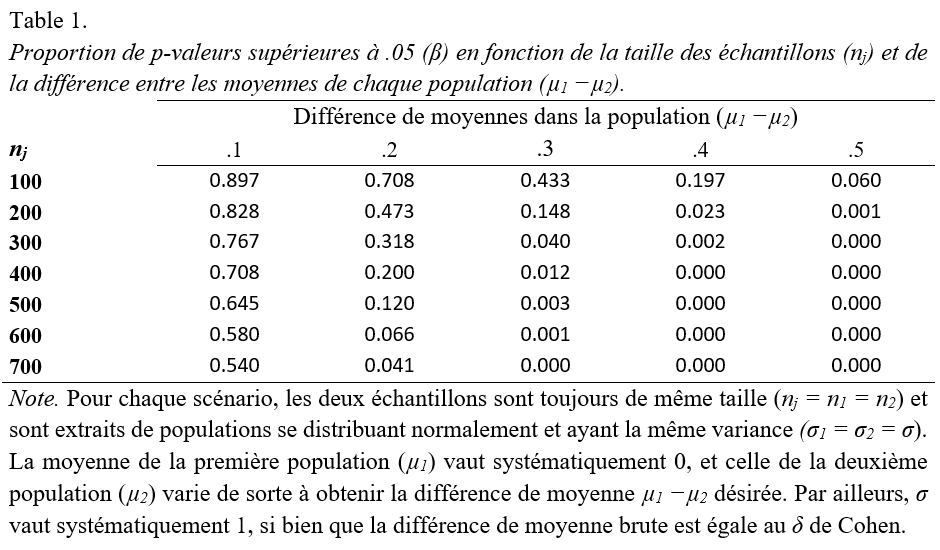
\includegraphics[width=1\linewidth]{C:/Users/Admin/Documents/Github projects/thesis/Chapitre 5/Illustration/Table1} \end{flushleft}
\newpage

Dans la mesure où une vraie différence entre les moyennes de population existe pour l'ensemble des scénarios envisagés dans la Table 1, nous espérerions être en mesure de rejeter l'hypothèse nulle le plus souvent possible. Pourtant, pour plusieurs scénarios, le nombre d'itérations amenant à conclure au non rejet de l'hypothèse nulle est bien supérieur au nombre d'itérations amenant à conclure au rejet de l'hypothèse nulle, comme on peut le voir à travers les valeurs \(\beta\) très élevées dans certains cas. Par exemple, avec 10 sujets par groupes et considérant \(\sigma_1=\sigma_2=1\), on ne détectera pas une différence de moyenne de .1 dans près de 95\% des cas. Avec 200 sujets par groupe, on ne détectera toujours pas cette différence dans plus de 80\% des cas. En présence d'un effet non nul, cela se justifie par un manque de puissance des tests réalisés, ce qui démontre bien qu'un non rejet de l'hypothèse nulle peut en fait signifier deux choses: soit qu'il n'y a vraiment pas de différence entre les moyennes des populations (ou autrement dit, que les différences observées sont dûes au hasard), soit que le test n'est pas suffisamment puissant pour détecter la différence. Or, le manque de puissance des tests est récurrent dans la littérature, comme tendent à le montrer diverses méta-analyses (\textbf{button\_power\_2013?}; \textbf{bakker\_rules\_2012?}; \textbf{funder\_improving\_2014?}).

Pour éviter d'interpréter un test peu puissant comme un soutien en faveur de l'hypothèse nulle, l'approche de la puissance est devenue l'approche par défaut dans les années 80 pour tester l'équivalence (\textbf{meyners\_equivalence\_2012?}). A travers cette approche qui est restée très populaire (\textbf{quertemont\_how\_2011?}), dans un premier temps, on définit ce qu'on considère comme étant la plus petite valeur d'intérêt (en anglais, le ``SESOI'' pour ``Smaller Effect Size of Interest''), c'est-à-dire la taille d'effet minimale requise pour considérer qu'un effet est pertinent. Ensuite, on estime la puissance de notre test à détecter un effet de cette taille\footnote{On parle d'estimation et non de mesure, car la puissance dépend de paramètres de population qu'on ne connait pas (Schuirmann,1987).}, et si cette estimation atteind une valeur jugée satisfaisante (en général, 80\%), alors on considère que l'on peut interpréter le non rejet de l'hypothèse nulle d'absence d'effet comme soutien en faveur de l'équivalence (\textbf{quertemont\_how\_2011?}; \textbf{meyners\_equivalence\_2012?}; \textbf{schuirmann\_comparison\_1987?}). L'idée sous-jacente est que si l'effet est au moins aussi grand que les limites de la zone d'équivalence, on devrait rejeter l'hypothèse nulle dans la majorité des cas. Par conséquent, un non rejet de l'hypothèse nulle devrait vraisemblablement signifier que l'effet n'atteint pas le SESOI et donc, que l'effet observé n'est pas pertinent.

Bien que ce raisonnement puisse sembler tentant, de prime abord, il présente d'importantes limites. Pour commencer, via cette approche, la probabilité de détecter une absence d'effet va augmenter quand la taille des échantillons va diminuer (\textbf{seaman\_equivalence\_1998?}). Afin de l'illustrer, nous avons créé la Table 2, dans laquelle nous envisageons les mêmes scénarios que pour la Table 1 et ajoutons une contrainte de puissance: nous considérons qu'il est nécessaire, pour pouvoir conclure à l'équivalence, d'atteindre une puissance de 80\% pour détecter une différence de moyenne de .1. Comme on peut le voir \emph{détailler un peu}.

, mais également quand l'erreur (la variabilité des scores au sein de chaque groupe) va augmenter (\textbf{meyners\_equivalence\_2012?}; \textbf{schuirmann\_comparison\_1987?}). Ce dernier point est illustré au sein de la Figure \ref{fig:schuirman2}, dans le contexte de la comparaison de deux moyennes. Sur l'axe des abscisses, on représente différentes estimations de la différence de moyenne (\(\bar{X_1}-\bar{X_2}\)) et sur l'axe des ordonnées, la précision des estimations \(\bar{X_1}-\bar{X_2}\) (\(S\sqrt{\frac{2}{n}}\) correspond à l'estimation de l'erreur standard de \(\bar{X_1}-\bar{X_2}\), avec \(S\) étant l'écart-type poolé et \(n\) la taille de chaque échantillon, lorsque les échantillons ont tous les deux la même taille et sont extraits de population ayant la même variance)\footnote{Par facilité, à l'instar de Schuirman (1987), on envisage le cas où les échantillons sont de même taille et que l'on suppose que la condition d'homogénéité des variances est respectée. Notons cependant que d'après Schuirman, ce raisonnement peut être généralisé aux scénarios où les deux échantillons n'ont pas la même taille et sont extraits de population n'ayant pas la même variance.}. Le triangle grisé représente l'ensemble des combinaisons estimation/précision qui vont amener à conclure à l'équivalence, avec l'approche de la puissance, lorsqu'on travaille avec des échantillons de taille 50, en acceptant un risque \(\alpha\) de 5\% et en exigeant une puissance minimale de 80\% pour détecter une différence de 20 unités (\(|\theta_j=20|,\;j=1,2\)). Dans cet exemple, pour toutes les valeurs de \(S\sqrt{\frac{2}{n}}\) supérieures à 7.07 aucune estimation de différence de moyennes ne permettra de conclure à l'équivalence (pas même 0) puisque la puissance du test à détecter une différence de 20 unités est inférieure à 80\%. Pour toutes les valeurs de \(S\sqrt{\frac{2}{n}}\) inférieures à 7.07, on constate que plus notre estimation de \(\bar{X_1}-\bar{X_2}\) est précise (lorsqu'on se déplace du haut vers le bas, sur l'axe des ordonnées), plus l'estimation doit être proche de 0 pour pouvoir conclure à l'équivalence. Cette propriété, peu désirable, n'est pas partagée par les tests d'équivalence dont fait partie le TOST que nous allons décrire ci-dessous (\textbf{schuirmann\_comparison\_1987?}).

\begin{figure}

{\centering 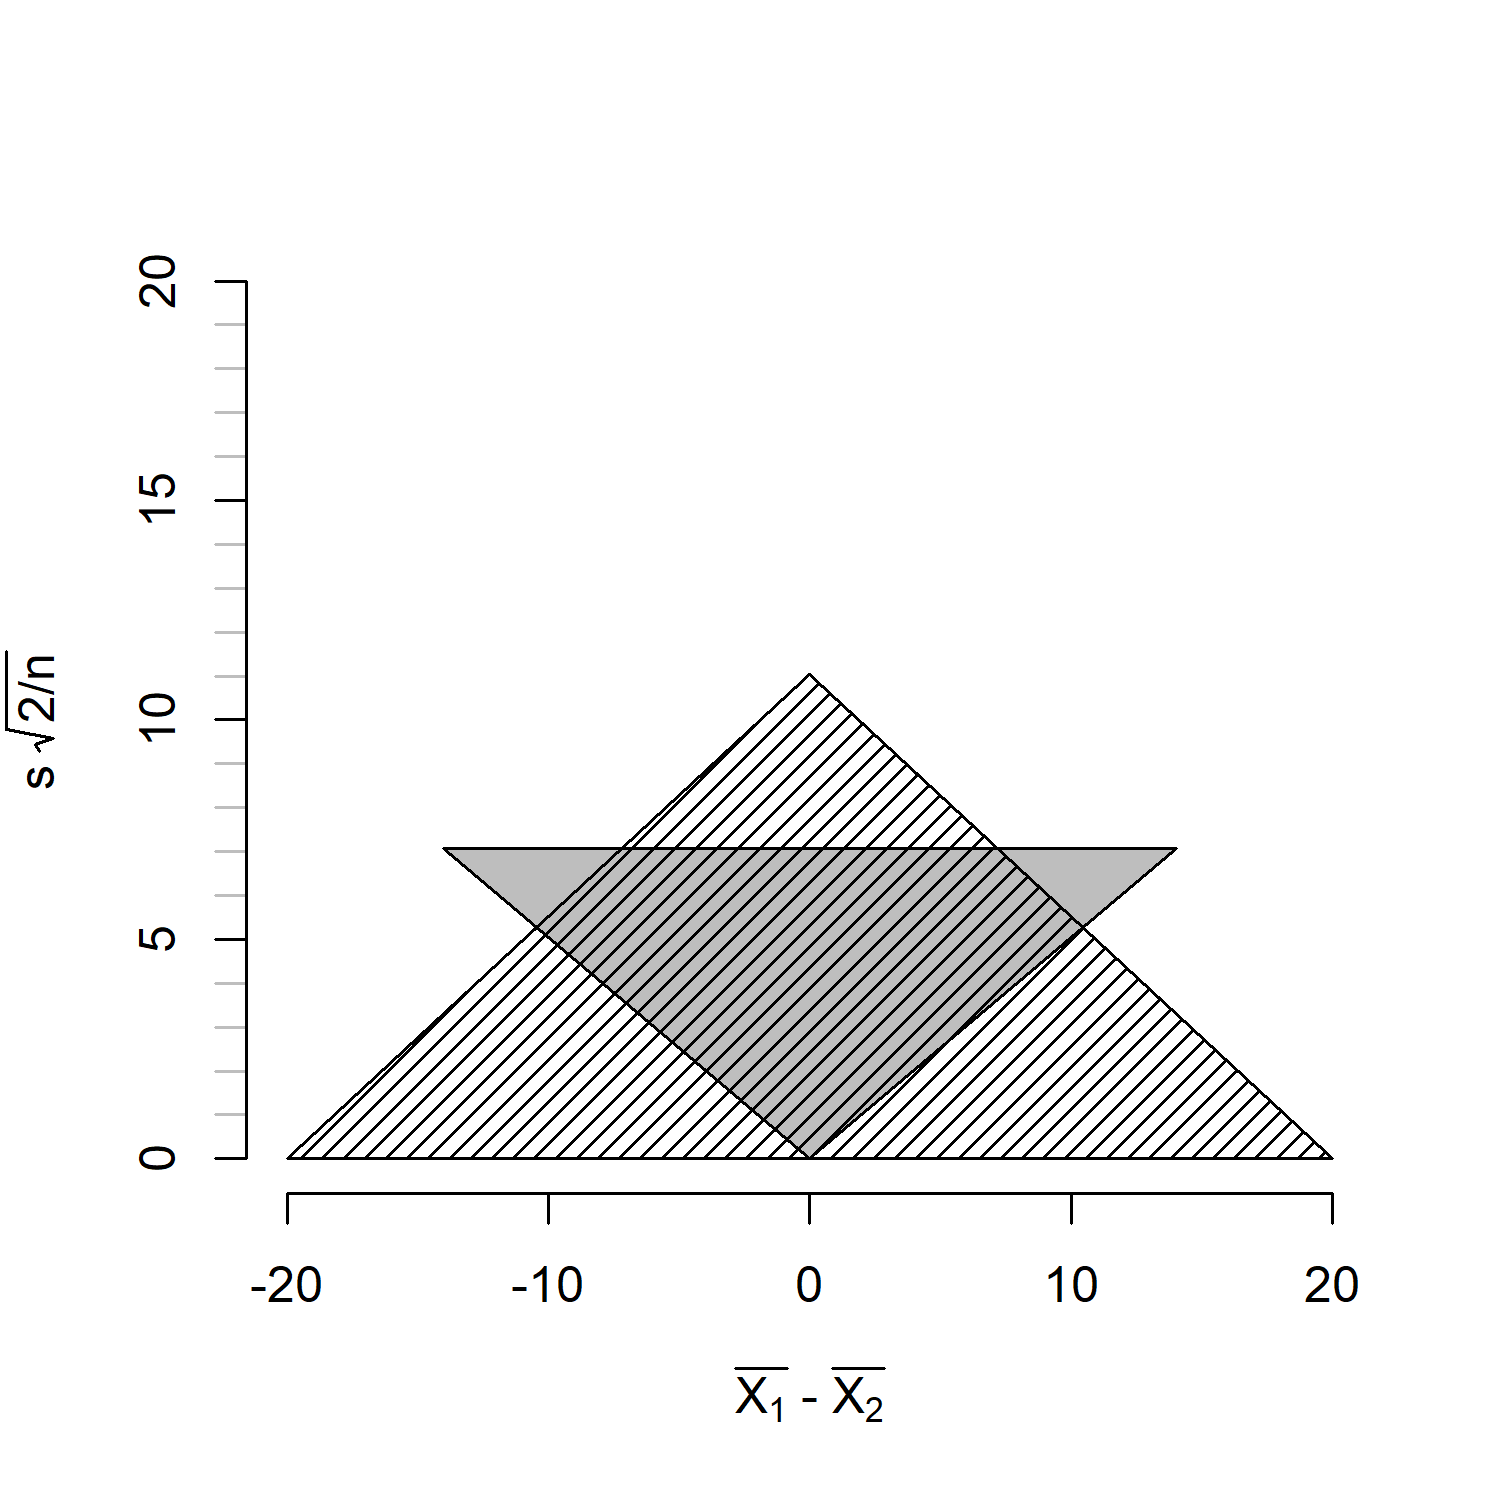
\includegraphics[width=0.96\linewidth]{C:/Users/Admin/Documents/Github projects/thesis/Chapitre 5/Illustration/Fig1} 

}

\caption{Région d'équivalence pour l'approche de la puissance (zone grisée) et pour le TOST (zone hachurée), pour l'exemple où $|\theta$|=20, n = 50 et $\alpha=.05$}\label{fig:schuirman2}
\end{figure}

\hypertarget{les-tests-duxe9quivalence}{%
\subsection{Les tests d'équivalence}\label{les-tests-duxe9quivalence}}

Avec les tests d'équivalence, il n'est pas possible de démontrer qu'un effet vaille exactement zéro (\textbf{meyners\_equivalence\_2012?}). Il est par contre possible de montrer que l'effet observé est suffisamment petit pour être jugé non pertinent. Or, cela peut s'avérer précieux dans de nombreuses situations, par exemple pour justifier la décision de regrouper plusieurs groupes de sujets ensemble (\textbf{rogers\_using\_1993?}), pour contrôler qu'il n'y ait pas de différence trop importante entre les groupes sur base de critères autres que le (ou les) facteur(s) d'intérêts en cas de quasi-expérience (\textbf{seaman\_equivalence\_1998?}) ou encore pour falsifier une théorie qui prônerait en faveur d'un effet dépassant une certaine taille (\textbf{lakens\_equivalence\_2017?}; \textbf{anderson\_theres\_2016?}).

Le point de départ des tests d'équivalence est de définir \(\theta_1\) et \(\theta_2\), les limites inférieures et supérieures de la zone d'équivalence, cette dernière contenant l'ensemble des valeurs jugées trop petites pour être susceptibles de nous intéresser. Ces limites peuvent être exprimées soit dans l'unité des données brutes, soit en terme standardisé, mais doivent être définies avant la récolte des données (\textbf{anderson\_theres\_2016?}). Il existe ensuite plusieurs approches pour démontrer que l'effet observé se situe dans la zone d'équivalence (voir \textbf{meyners\_equivalence\_2012?}, par exemple). Parmis celles-ci, une approche très simple est celle du ``Two one-sided tests'' (\textbf{schuirmann\_comparison\_1987?}; \textbf{lakens\_equivalence\_2017?}), plus communément appelé le TOST \footnote{Il existe des alternatives au TOST qui sont très légèrement plus puissantes, mais le gain marginal en termes de puissance est contrebalancé par un niveau de complexité beaucoup plus élevé (Meyners, 2012).}. Le principe est de définir deux hypothèses nulles. La première est que l'effet observé est inférieur à la limite inférieure de la zone d'équivalence: \[\it H0_1: \theta < \theta_1, \; avec \; \theta_1 \neq 0\] La deuxième est que l'effet observé est supérieur à la limite supérieure de la zone d'équivalence: \[\it H0_2: \theta > \theta_2, \; avec \; \theta_2 \neq 0\] Lorsque les deux hypothèses nulle peuvent être simultanément rejetées, on peut conclure à l'équivalence (\textbf{seaman\_equivalence\_1998?}). Cela équivaut, statistiquement parlant, à montrer que l'intervalle de confiance à \((1-2\times\alpha)\%\) est entièrement inclus dans la zone d'équivalence (\textbf{seaman\_equivalence\_1998?}; \textbf{lakens\_equivalence\_2017?}). Notons qu'il n'est pas nécessaire de reporter les résulats des deux tests unilatéraux, lorsqu'on réalise le TOST: il suffit de reporter les résultats du test associé à la plus petite valeur de statistique (et par conséquent, à la plus grande \(p\)-valeur). En effet, si ce test amène à conclure au rejet de l'hypothèse nulle, le second test amènera automatiquement à la même conclusion (\textbf{rogers\_using\_1993?}; \textbf{lakens\_equivalence\_2018?}). Cette remarque reste vraie dans le cas particulier où les deux tests sont associés à la même valeur de statistique puisque dans ce cas, les deux tests mèneront à une conclusion identique (\textbf{rogers\_using\_1993?}). Notons également qu'il n'est pas nécessaire de procéder à une correction du risque alpha dûe à la réalisation simultanée de deux tests. En effet, une erreur de type I (rejeter à tort l'hypothèse nulle) ne peut être commise que si l'hypothèse nulle est vraie. Or, les deux hypothèses nulles testées sont mutuellement exclusives: il n'est pas possible que \(\theta\) soit simultanément inférieur à \(\theta_1\) (ce qui correspond à \(\it H0_1\)) et supérieur à \(\theta_2\) (ce qui correspond à \(\it H0_2\)).

\begin{figure}

{\centering 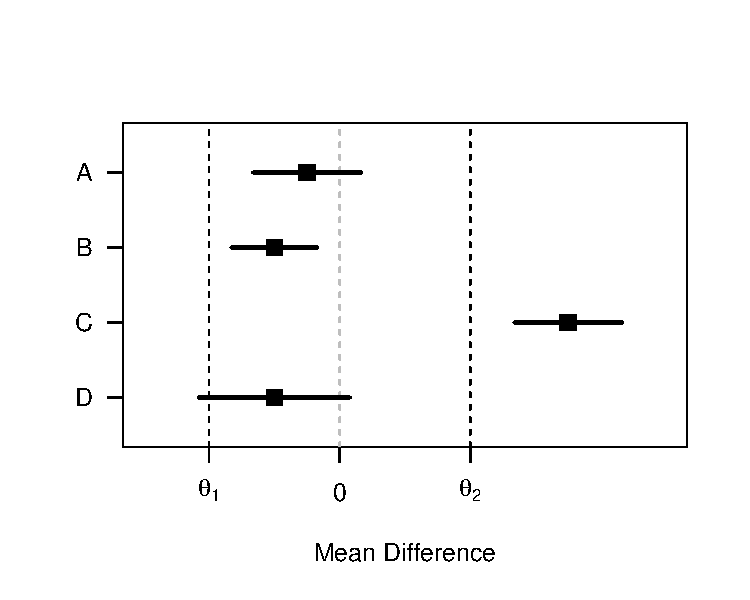
\includegraphics{chp5_files/figure-latex/equiv1-1} 

}

\caption{Différence de moyennes ($\bar{X_1}-\bar{X_2}$) et IC à $1-2\alpha\%$ autour de la différence de moyennes ($\bar{X_1}-\bar{X_2}$) pour 4 scénarios distincts.}\label{fig:equiv1}
\end{figure}

Jusqu'il y a peu, le TOST n'était pas disponible dans la plupart des logiciels, à l'exception de Minitab, ce qui constituait un frein important à son usage. Pour cette raison, (\textbf{lakens\_20\_2016?}) a créé le package TOSTER et plus récemment encore, ce même package a été implémenté dans Jamovi \footnote{Jamovi est un logiciel clic-bouton entièrement gratuit qui gagne en popularité et qui présente, parmi ses nombreux avantages, le fait d'être très convivial. Dans la mesure où la plupart des chercheurs sont plus enclins à utiliser des procédures si elles sont implémentées dans ce type de logiciel (Fraas $\&$ Newman, 2000), cela constitue une excellente nouvelle pour le devenir du TOST dans la recherche en psychologie.}. Tant dans R que dans Jamovi, le package TOSTER compare simultanément l'effet observé à 0 (test traditionnel d'absence d'effet) ainsi qu'aux deux bornes de la zone d'équivalence (TOST). Il en découle 4 conclusions distinctes possibles (\textbf{lakens\_equivalence\_2017?}), qui sont illustrées dans la figure \ref{fig:equiv1} dans le contexte de la comparaison de deux moyennes indépendantes:

\newpage

\begin{enumerate}
\def\labelenumi{(\arabic{enumi})}
\item
  Les résultats du TOST sont statistiquement significatifs, mais pas celui du test traditionnel d'absence d'effet (scénario A, Figure \ref{fig:equiv1}): dans ce cas, on conclura à l'absence d'effet ayant un quelconque intérêt pratique (\textbf{rogers\_using\_1993?}).
\item
  Tant les résultats du TOST que du test traditionnel sont significatifs (scénario B, Figure \ref{fig:equiv1}): on conclura alors qu'il existe un effet non nul, mais que celui-ci est si petit qu'il ne présente aucun intérêt pratique. C'est ce qui arrive typiquement lorsqu'on travaille avec de très grands échantillons, si bien que le test traditionnel est très puissant, même pour détecter des effets très petits (\textbf{rogers\_using\_1993?}).
\item
  Le résultat du test traditionnel est statistiquement significatif, mais pas ceux du TOST (scénario C, Figure \ref{fig:equiv1}): on conclura alors à la présence d'un effet non nul (\textbf{rogers\_using\_1993?}).
\item
  Ni les résultats du TOST, ni celui du test traditionnel n'est statistiquement significatif (scénario D, Figure \ref{fig:equiv1}): c'est ce qui arrive lorsque les données sont si imprécises qu'on ne peut tirer aucune conclusion. Les données semblent compatibles tant avec un effet nul qu'avec un effet au là des bornes d'équivalence.
\end{enumerate}

\hypertarget{duxe9finir-les-limites-de-la-zone-duxe9quivalence}{%
\subsection{Définir les limites de la zone d'équivalence}\label{duxe9finir-les-limites-de-la-zone-duxe9quivalence}}

L'aspect le plus compliqué dans la réalisation du TOST est la définition des bornes d'équivalence. Il existe plusieurs stratégies pour établir des bornes. L'idéal est la situation où il est possible de définir un critère objectif qui permettra de déterminer à partir de quand un effet est jugé pertinent (Lakens et al.~2018). \emph{Exemple: augmentation de la rougeur de la peau pendant les règles qui aurait un impact sur la perception d'attractivité chez les hommes. Pour que ce soit vrai,il faut pouvoir montrer que le changement de rougeur de la peau soit détectible à l'oeil nu. Il est alors possible de définir là un critère objectif}. Mais ce n'est malheureusemnt pas toujours le cas (surtout dans des domaines d'études tels que la psychologie). Lorsqu'il n'est pas possible d'établir un critère objectif, il existe plusieurs stratégies, plus subjectives qui vont permettre d'établir les bornes.\\
1) S'appuyer sur des benchmarks. Attention, bien que cette solution soit facile, son gros inconvénient et qu'elles ne prennent pas du tout en compte le contexte. \emph{Faire la remarque sur les benchmarks un peu mieux que celles de Cohen que j'ai fait sur le blog post de cumming.}
2) se baser sur des études antérieures (dans le contexte de réplication).
2.1. (Levine et al.~2007): se baser sur les tailles d'effet suggérées dans la littérature (sur base de méta-analyses)\footnote{Il est mieux de se baser sur des résultats de méta-analsye que d'étude isolée parce qu'à cause du biais de publication, les tailles d'effet observées sont souvent une sur-représentation de la réalité et donc si on a bcp de sujets dans notre étude, il y a vraiment bcp de chance qu'on démontre l'équivalence}.\emph{Prenons l'exemple de l'augmentation de la pensée agressive quand on joue à des jeux violents. D'après une méta-analyse de Ferguson (2007), cette corrélation serait de r =.25 (ce qui correspond à un d de Cohen de .51). Je peux utiliser cette valeur comme borne pour définir l'intervalle d'équivalence. Si je parviens à montrer qu'il y a équivalence, je montre que l'effet étudié serait vraisemblablement plus petit que suggéré dans la littérature. }.\\
--\textgreater{} Remarque: la méta-analyse elle donne .25, OK, mais en réalité, il y a une distribution autour de l'effet dans la littérature. Une solution plus conservatrice est alors de se baser sur les bornes inférieures de l'IC autour de la valeur de la méta-analyse.
--\textgreater{} Comme dit Vincent, c'est la réalité de l'effet. C'est comme si tu faisais un test entre deux moyennes en prétendant que la myenne est une valeur et pas une distribution autorud e cette effet. Et donc c'est un peu délicat d'aller dire qu'on va tester un test d'équivalence pour contester l'effet de la violence en prenant la valeur obtenue dans la méta analyse comme une borne absolue et pas une distribution. Du coup, au minimum il essayerait d'intégrer le fait qu'il y a une distribution autour de la valeur, mais donc on ne peut pas décider que si on est en dessous de .50 ou au dessus de -.50.\\
--\textgreater{} Autre probleme, pourquoi prendre l'opposé comme borne inférieure? Alors que la méta analyse ne parle pas d'effet inverse.
--\textgreater{} Pour l'heure, je serais plus d'avis de confirmer la méta-analyse en montrer que l'effet est bien situé à l'intérieur des bornes de l'IC autour de cet effet dans la méta-analyse.
2.2. Solution proposée par Simonsohn (2015) pour remettre en question la pertinence de l'outil qui a ét utilsié pour démontrer un effet dans une étude antérieure. Il dit que si on a pour un effet d'intérêt une puissance inférieure à 33\% de le détecter, on a vraiment un gros problème de puissance (pourquoi 33\% ça reste arbitraire, of course). il part de cette optique là et il se dit que du coup, ça pourrait être intérssant de définir les bornes de la zone d'équivalence en considérant un effet que l'étude d'origine aurait pu détecter avec une puissance de 33\%. Ce faisant, si on parvient à démontrer que l'effet est encore plus petit qu'un effet que l'étude ne base n'aurait pu détecter qu'avec une puissance de 33\%, il y a peu de chance pour que l'effet originellement proposé par l'étude d'origine soit vraiment basé sur un outil pertinent. \emph{exemple concrêt: imaginons un test t de Student et qu'on a 21 sujets par groupe. On peut déterminer, en faisant une analyse de sensibilité dans Gpower, qu'on a une puissance 33\% à détecter un effet d de COhen de .48. Du coup, on considererais .48 comme valeur pour notre zone d'équivalence.}\\
2.3. Lakens (2018): essayer de deviner implicitement ce que l'auteur de l'étude d'origine aurait pu considérer comme un effet pertinent (s'il n'a pas donné d'indication dans son article pour dire " je considère qu'un effet est pertinent à partir de telle valeur"). Cela peut se faire sur base de la taille d'échantillon utilisée par cette personne. \emph{On ne pourra détecter un effet comme significatif que si la valeur de statistique observée dépasse une valeur seuil (la valeur critique). Il est possible, grâce à la relation qui existe entre la statistique t et la statistique d de Cohen, de déterminer à quelle ``taille d'effet critique'' correspond la statistique t critique. Par exemple, si le chercheur a utilisé 30 sujets par groupe: via gpower, on peut déterminer qu'il faudra une statistique observée t de minimum 2.045 pour pouvoir conclure au RH0. et compte tenu du lien entre la statistique t et la stat d, ça correspond à un d de Cohen de .373 (d\_crit = t\_crit/racine(n)). Concrètement, si on observe une taille d'effet supérieure ou égale à .373, on pourra conclure au rejet de l'H0. Si la taille d'effet est plus petite, on ne sera pas capable de conclure au rejet de l'hypothèse nulle. L'idée ce serait de démontrer qu'il y a équivalence, la personne qui a écrit l'article d'origine a utilisé une taille d'échantillon insuffisante pour étudier l'effet suggéré et donc, si on veut étudier ce même sujet d'étude, il faudrait nécessairement récolter des échantillons plus grands pour être capable de le faire correctement. }

\begin{enumerate}
\def\labelenumi{\arabic{enumi})}
\setcounter{enumi}{2}
\tightlist
\item
  de se baser sur les ressources dont on dispose (analyse de sensibilité). Si moi je ne suis pas capable d'avoir un échantillon de plus de 2000 personnes, il y a certains effets que je ne serai pas capable de calculer. Et donc, je peux utiliser cette taille d'échantillon pour déterminer la taille d'effet dont je suis certain que je pourrai raisonnablement conclure au rejet de l'hypothèse nulle. Et donc là, si on démontre qu'il y a équivalence, on ne tire pas la ccl que l'effet n'est pas pertinent, mais que cet effet qu'on a envie d'étudier ne peut être l'être sur base des tailles d'échantillon qu'on a l'habitude d'utiliser.
\end{enumerate}

Il est important de bien comprendre qu'en fonction de la stratégie utilisée, on ne se posera pas nécessairement la même question de recherche (et la réponse obtenue sera nécessairement liée à cette question de recherche).

\begin{enumerate}
\def\labelenumi{\arabic{enumi})}
\tightlist
\item
  définir comme limites la plus petite taille d'effet pour laquelle on peut atteindre une puissance de détection suffisante (déterminé par les ressources disponibles pour étudier l'effet, (\textbf{lakens\_equivalence\_2017?})) --\textgreater{} voir la section ``Setting equivalence bounds'' p.~359 mais je crois que j'en parle aussi dans la vidéo SOCLAB.\\
\item
  le SESOI peut parfois être fixé objectivement
\item
  Idéalement basé sur une analyse coût-bénéfice). Attention: bien sûr une dimension subjective dans la définition des coûts et des bénéfices.
  Attention: le SESOI doit être déterminé AVANT et INDEPENDAMMENT des données.
\end{enumerate}

\hypertarget{comparaison-du-tost-et-du-sgpv}{%
\subsection{Comparaison du TOST et du SGPV}\label{comparaison-du-tost-et-du-sgpv}}

\begin{center}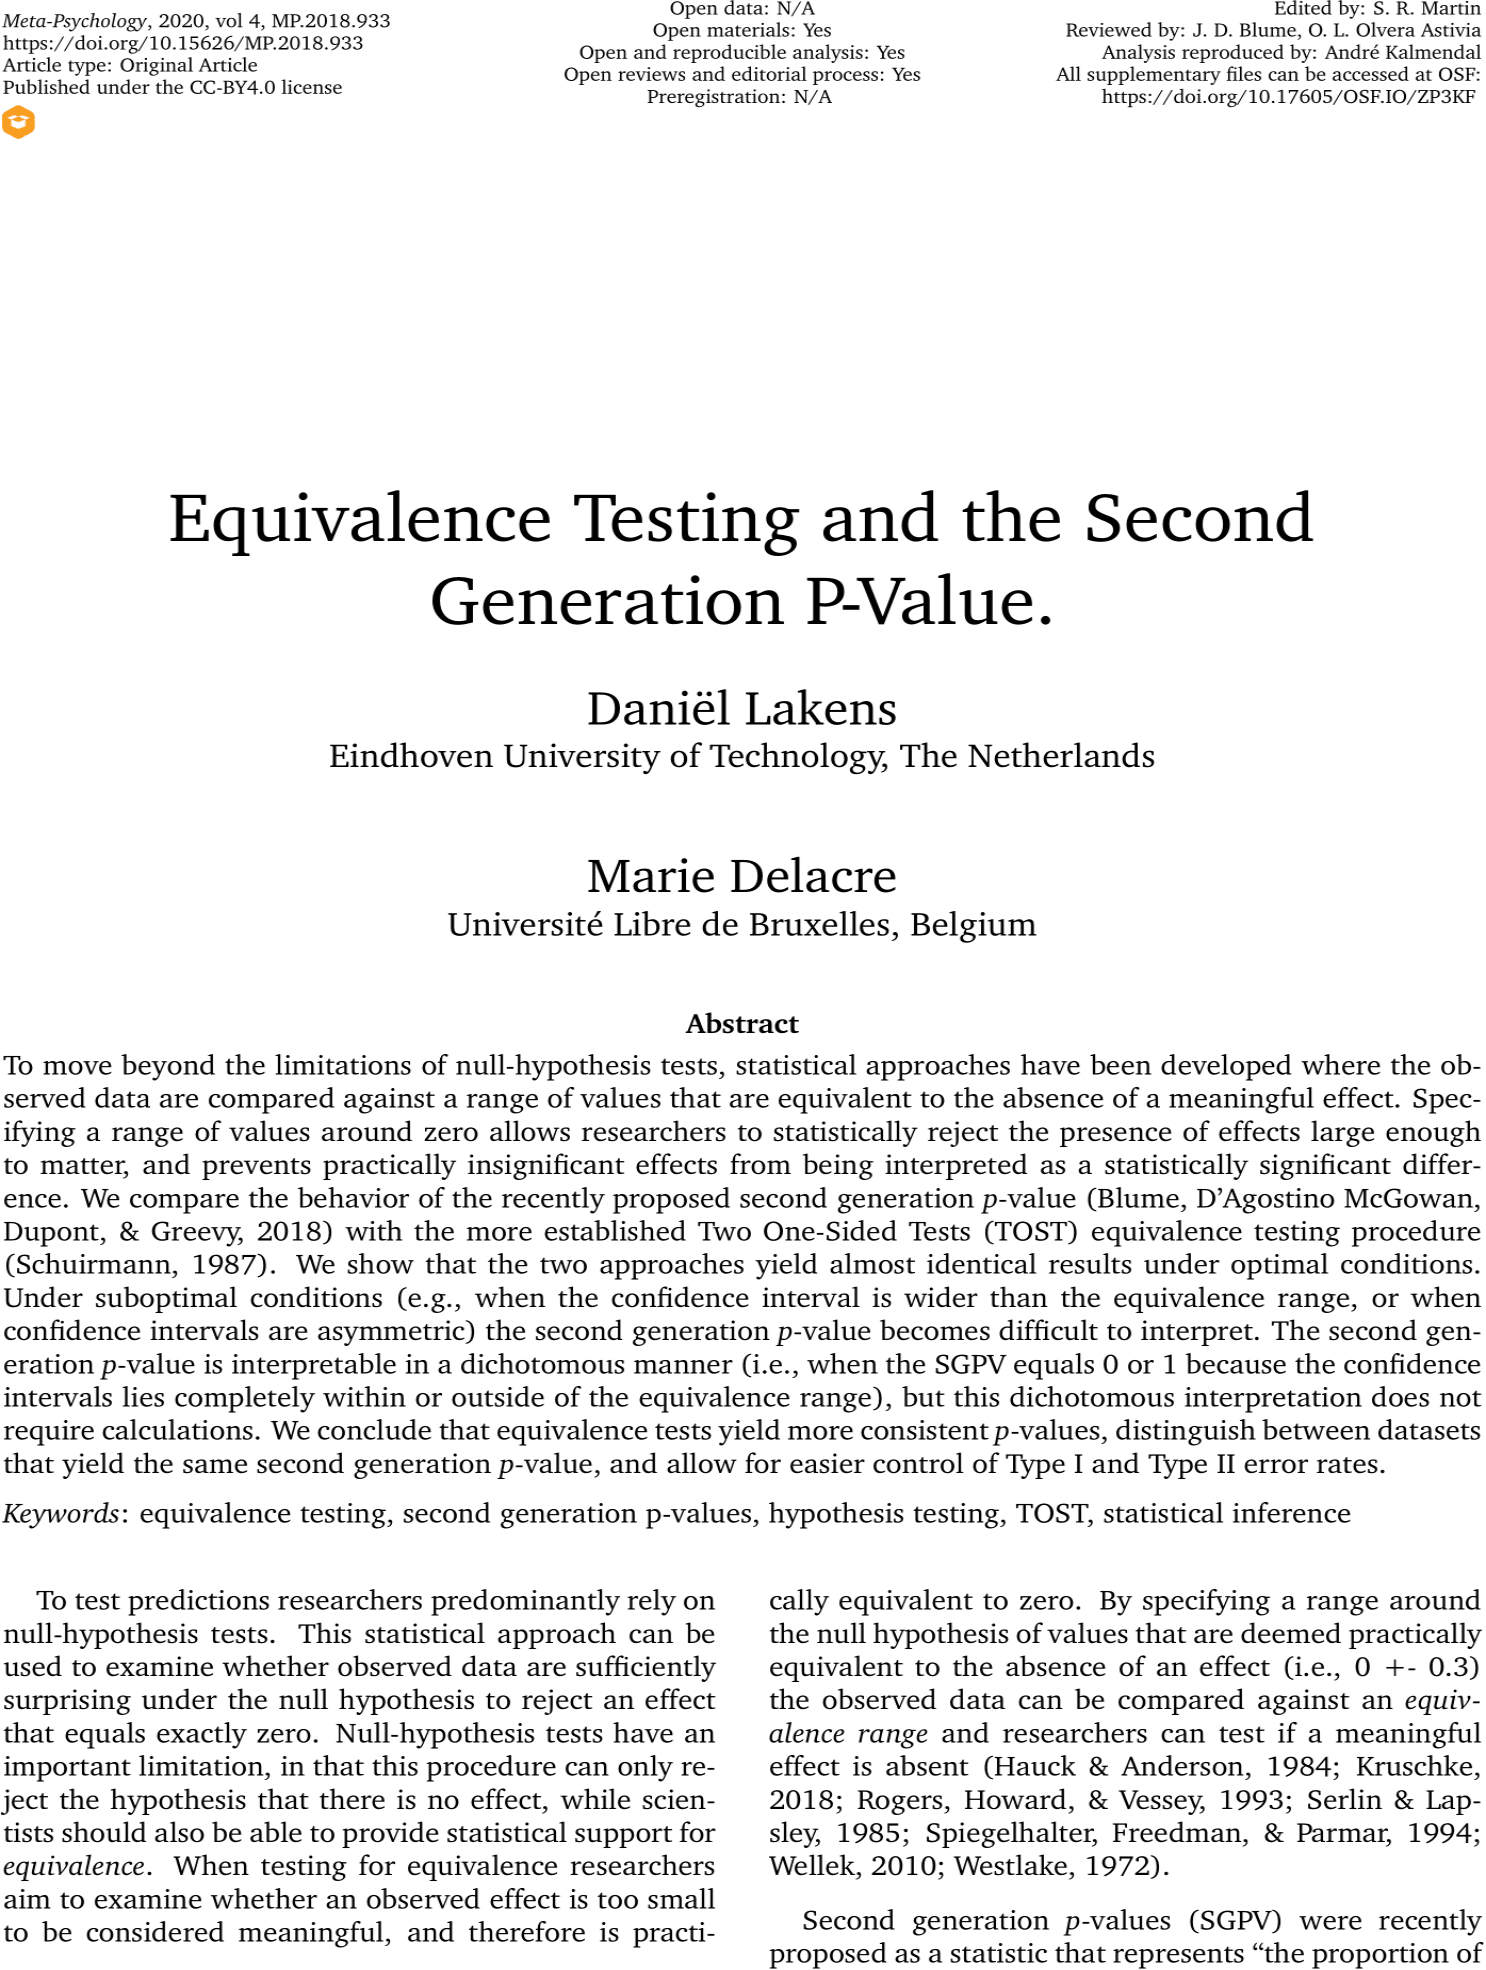
\includegraphics[width=0.92\linewidth]{C:/Users/Admin/Documents/Github projects/thesis/Chapitre 5/Chapitre 5-1} \end{center}

\begin{center}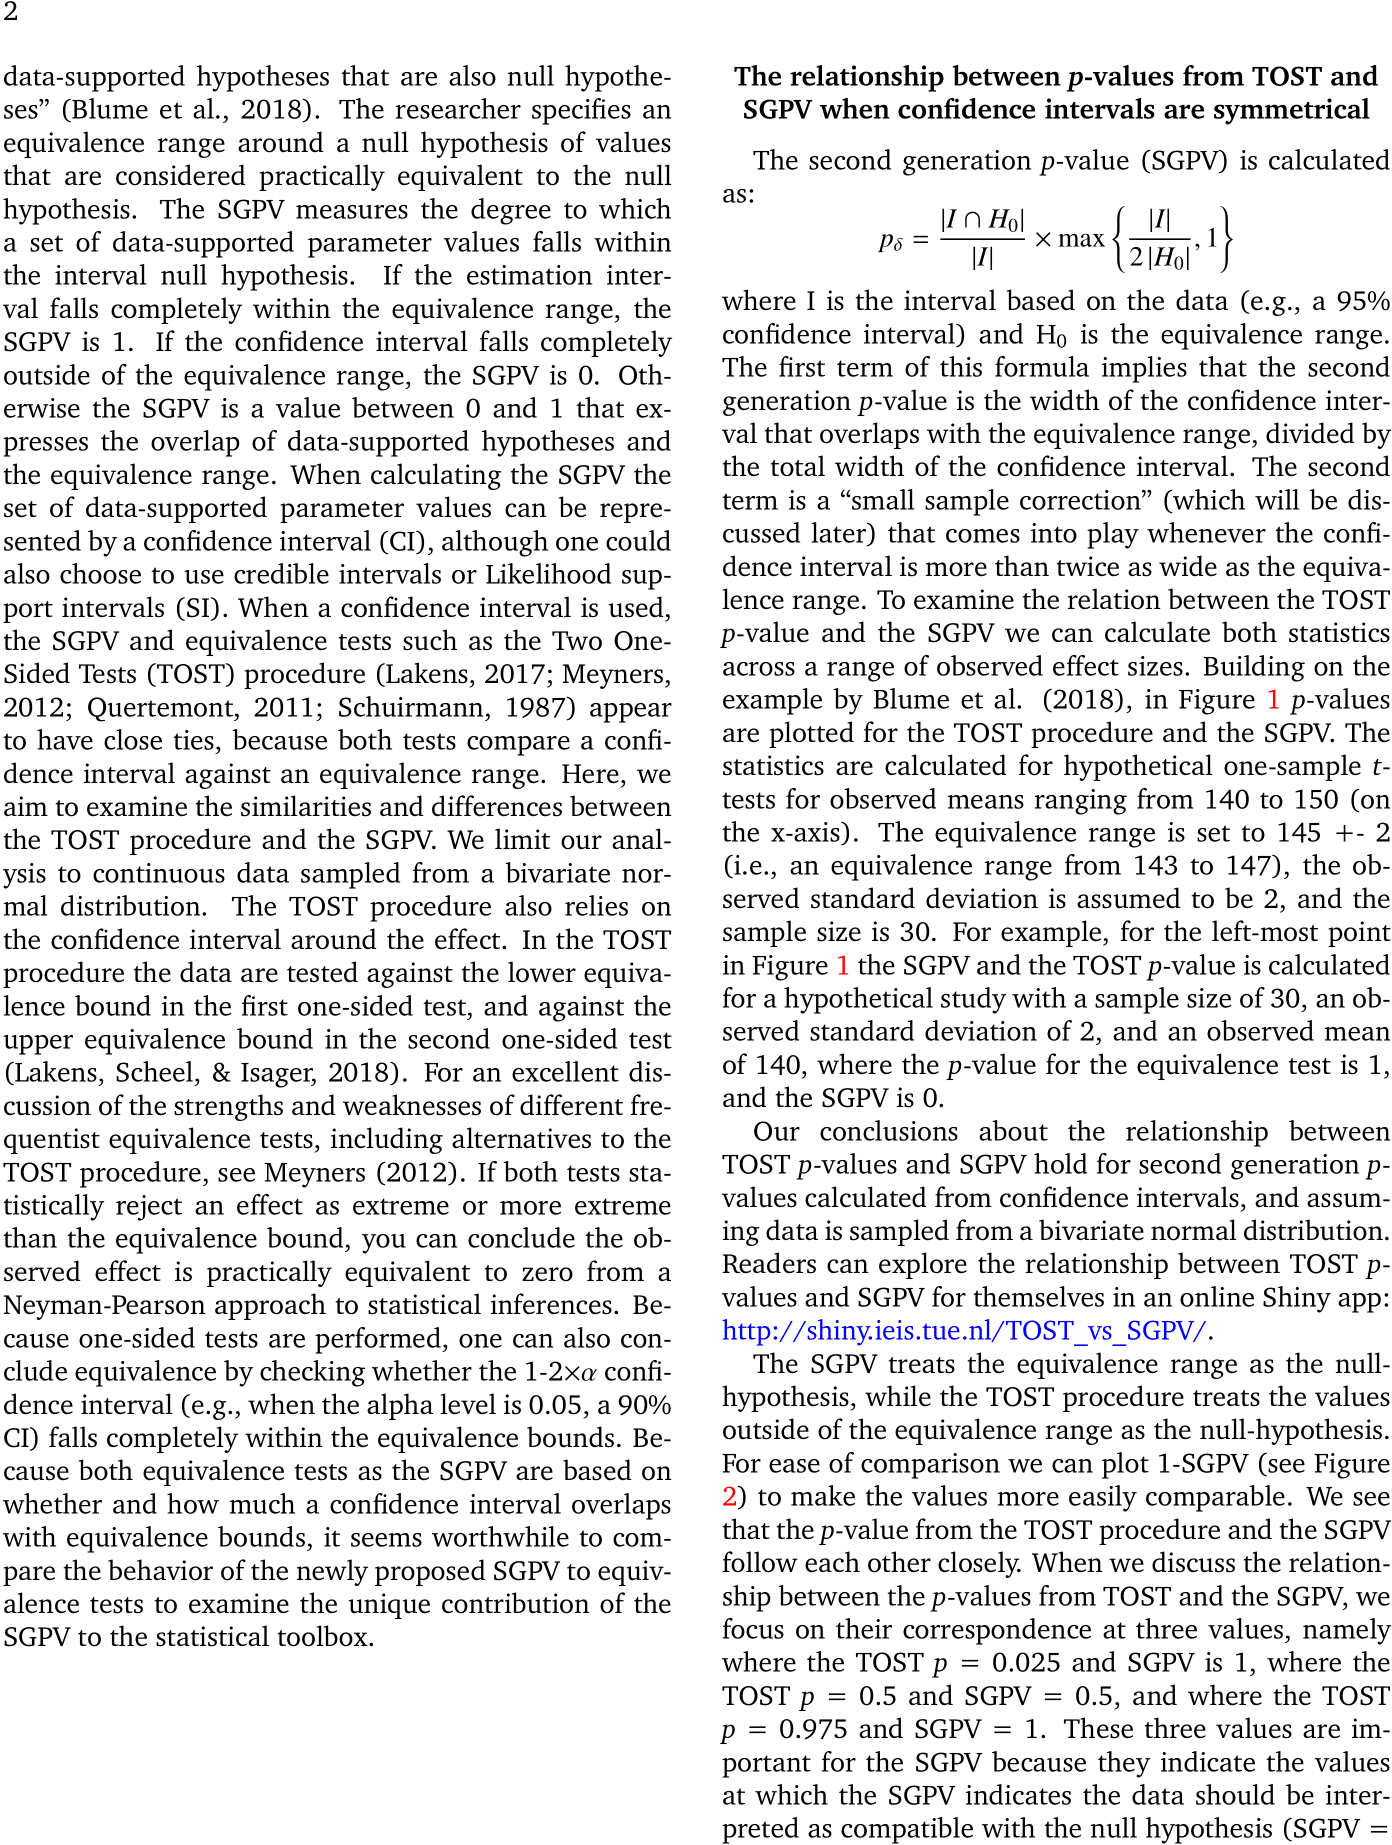
\includegraphics{C:/Users/Admin/Documents/Github projects/thesis/Chapitre 5/Chapitre 5-2} \end{center}

\begin{center}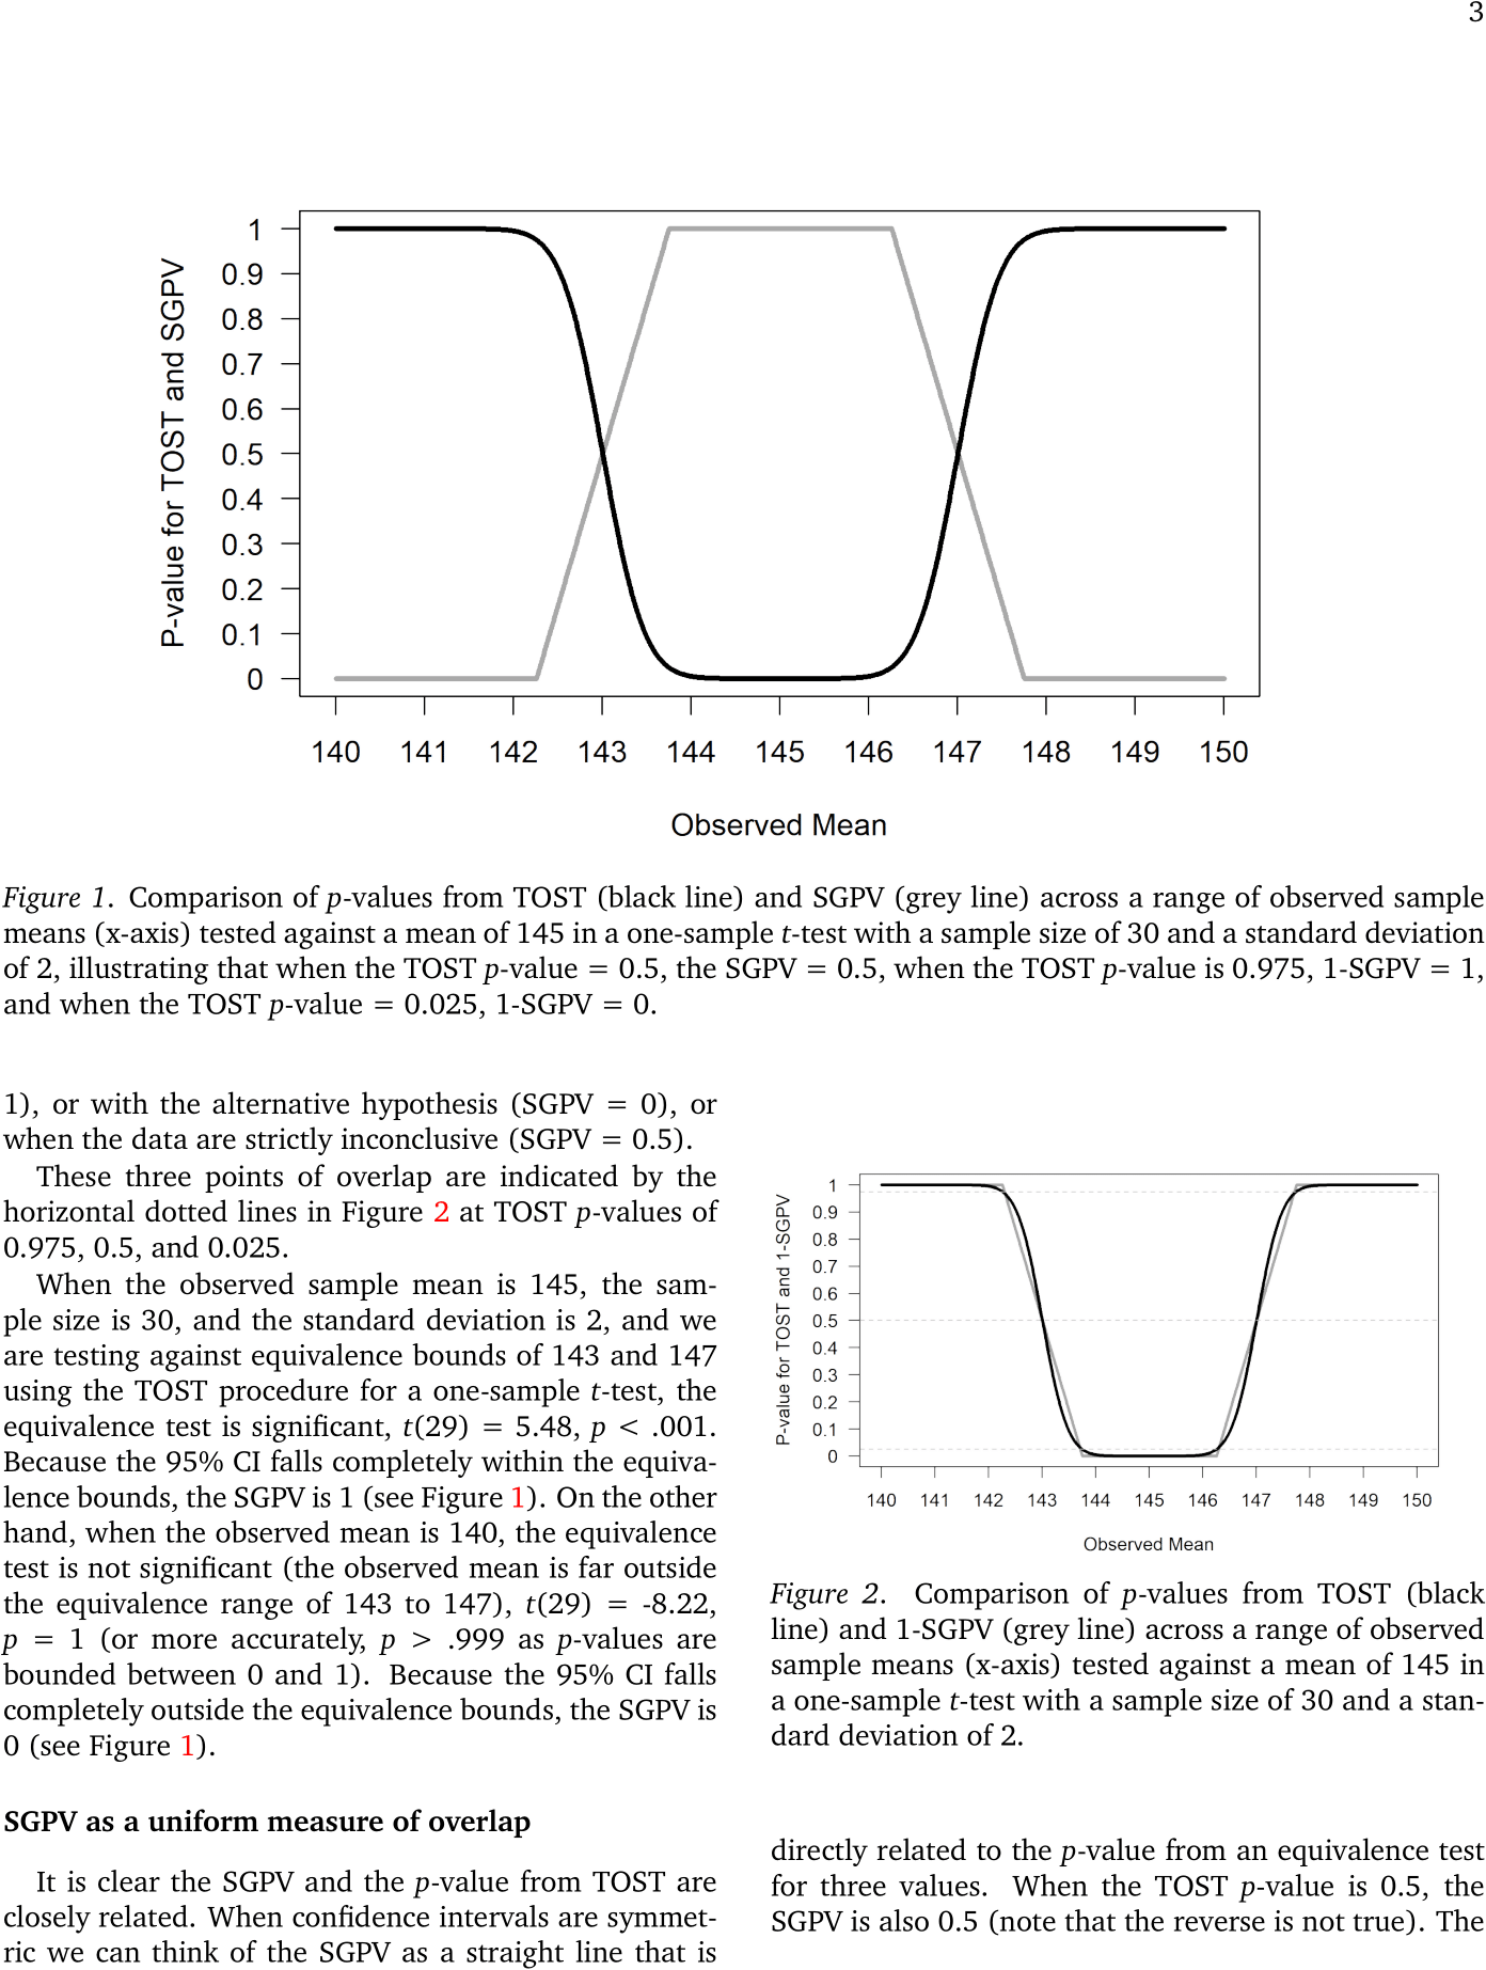
\includegraphics{C:/Users/Admin/Documents/Github projects/thesis/Chapitre 5/Chapitre 5-3} \end{center}

\begin{center}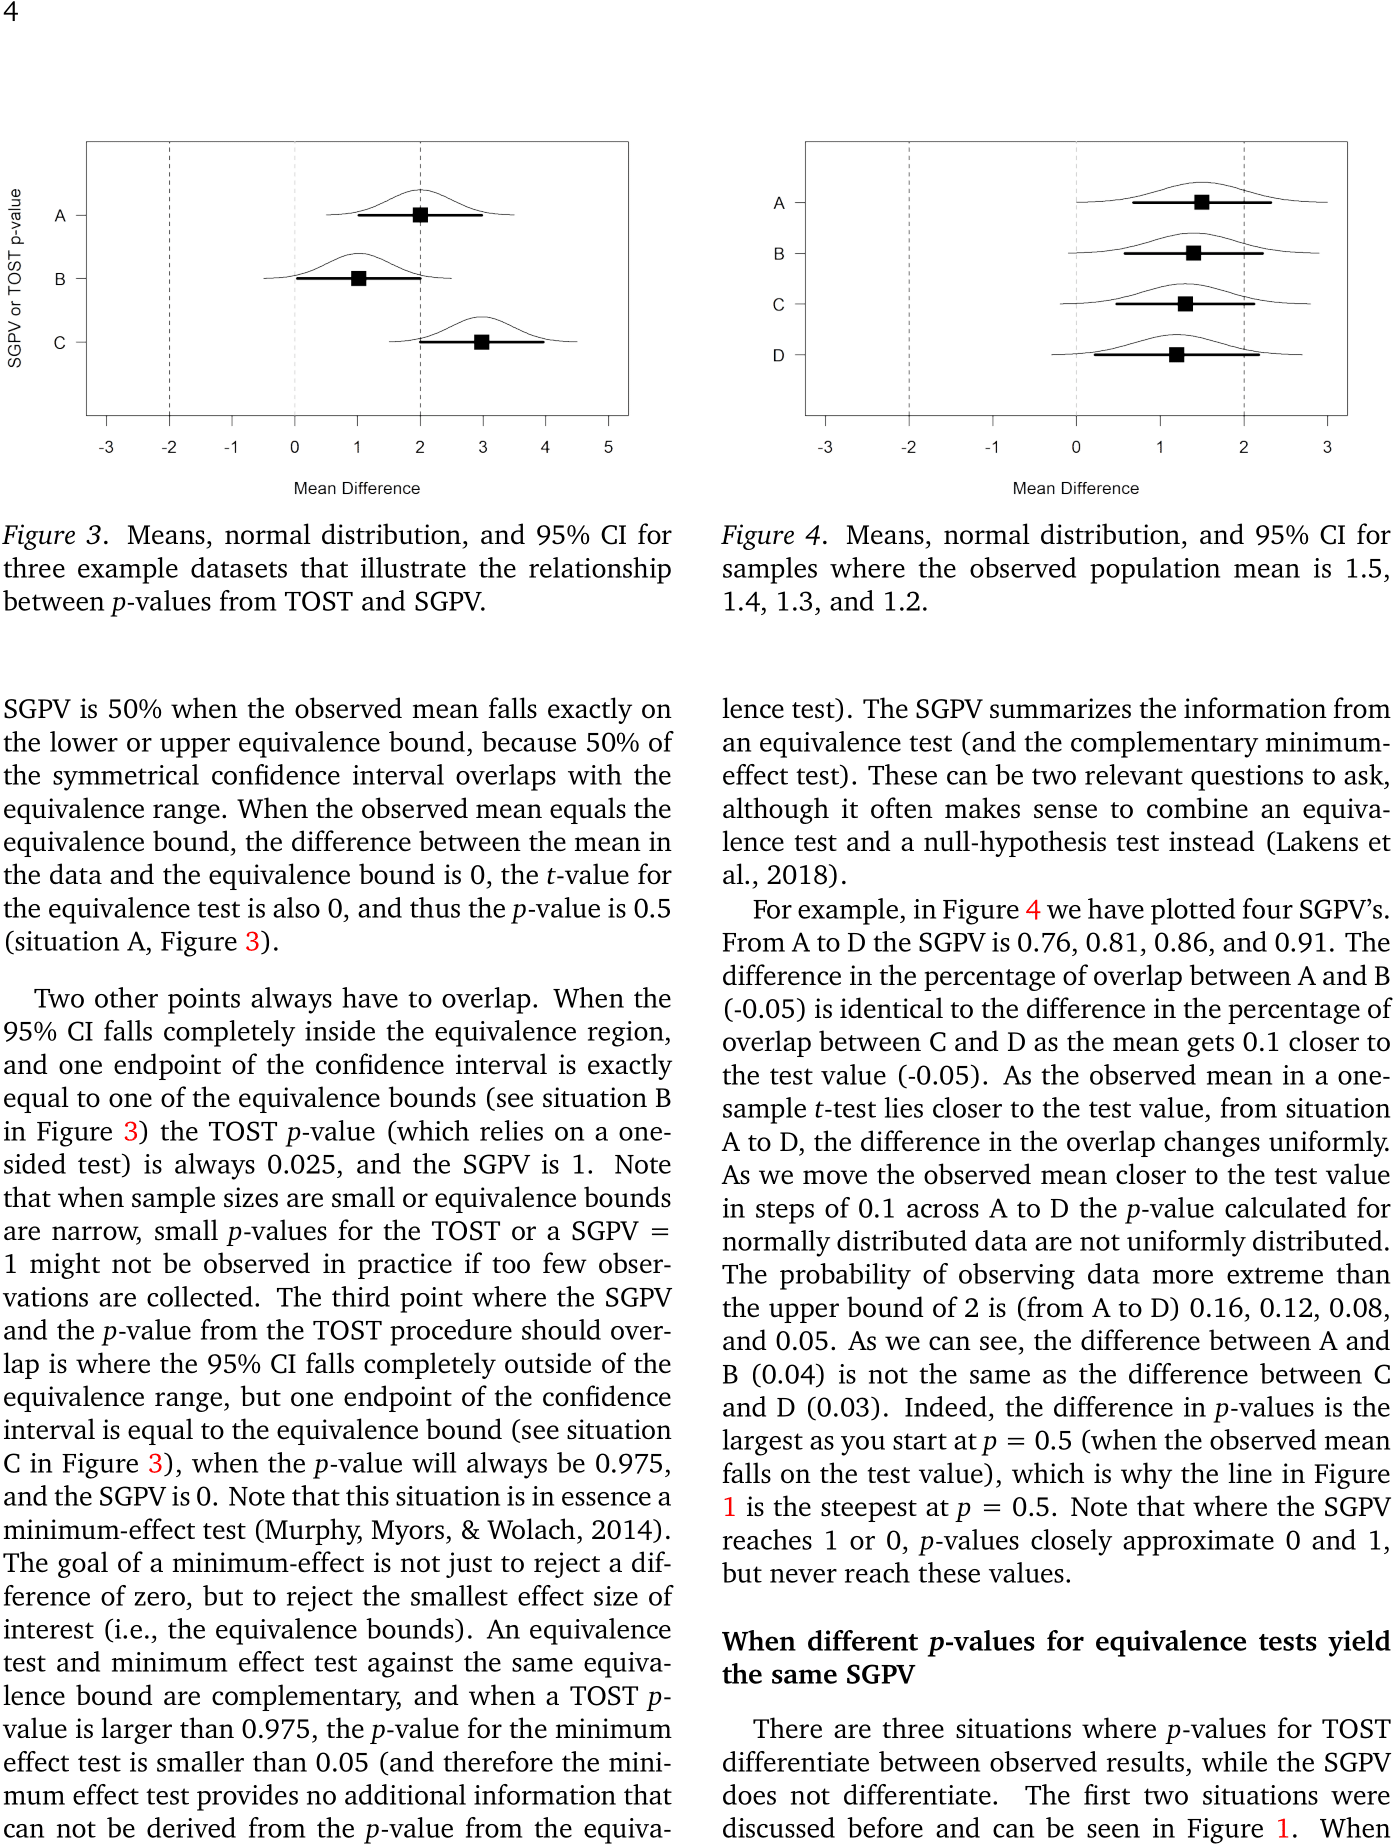
\includegraphics{C:/Users/Admin/Documents/Github projects/thesis/Chapitre 5/Chapitre 5-4} \end{center}

\begin{center}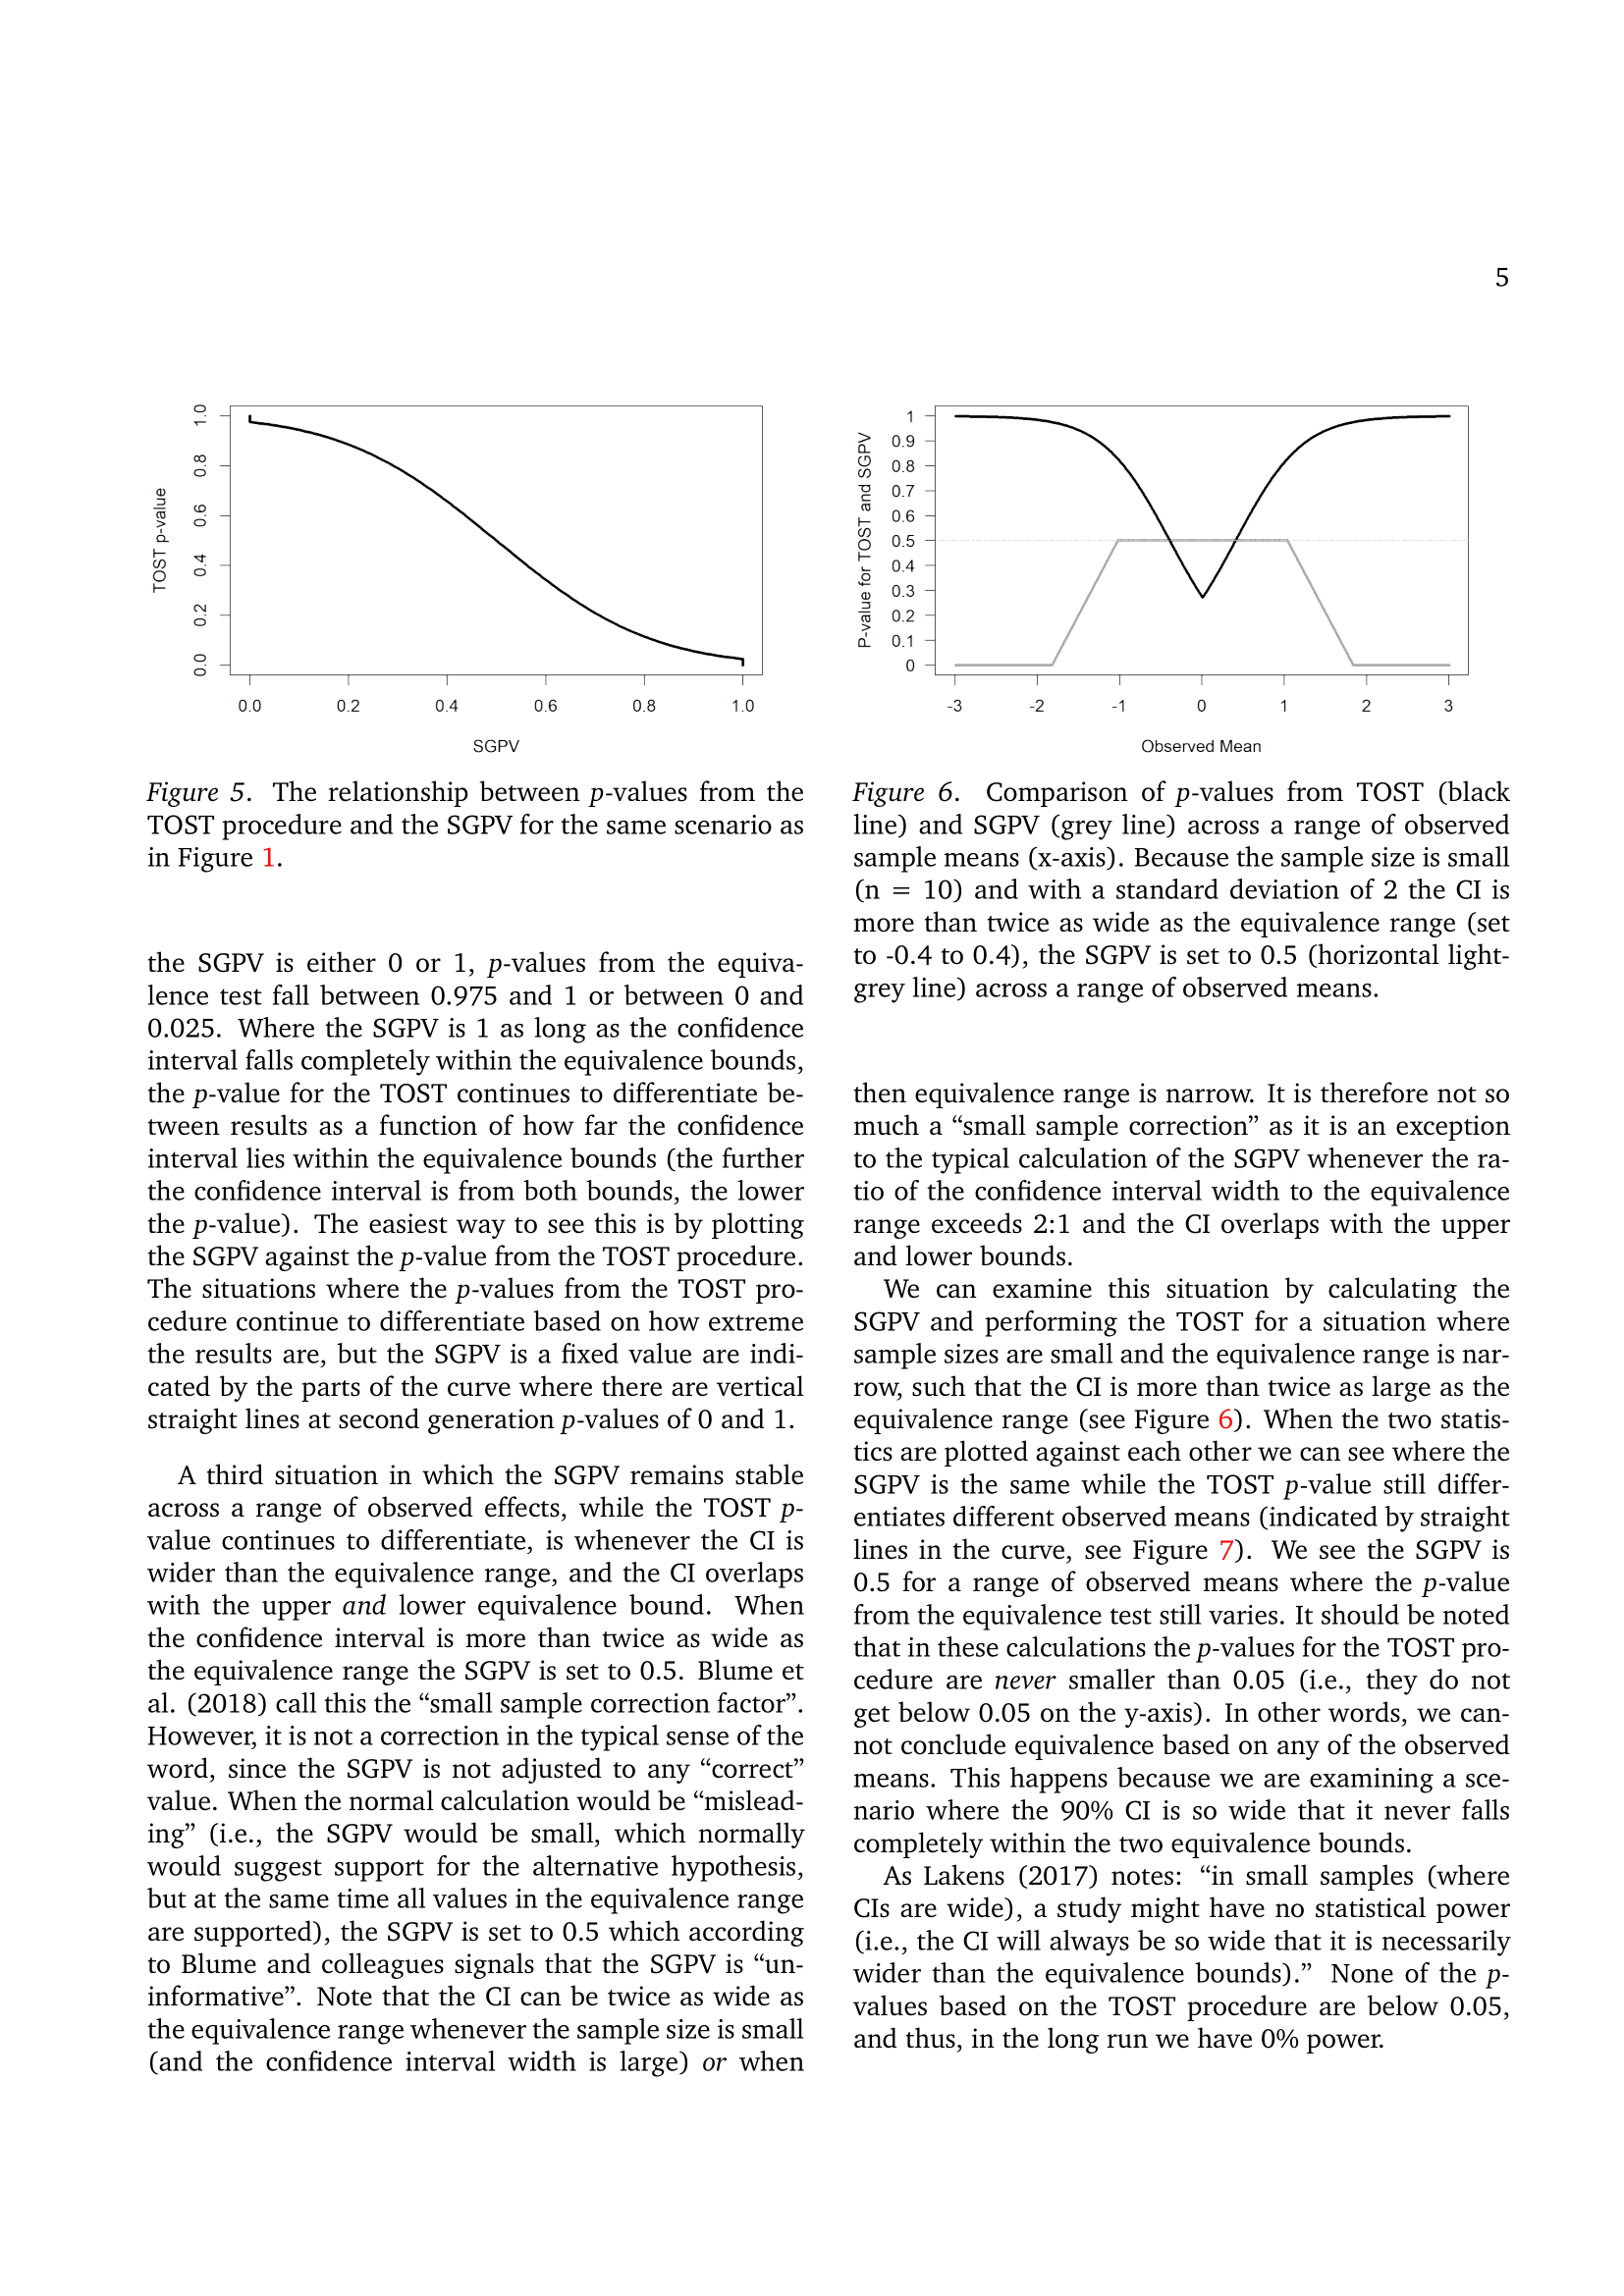
\includegraphics{C:/Users/Admin/Documents/Github projects/thesis/Chapitre 5/Chapitre 5-5} \end{center}

\begin{center}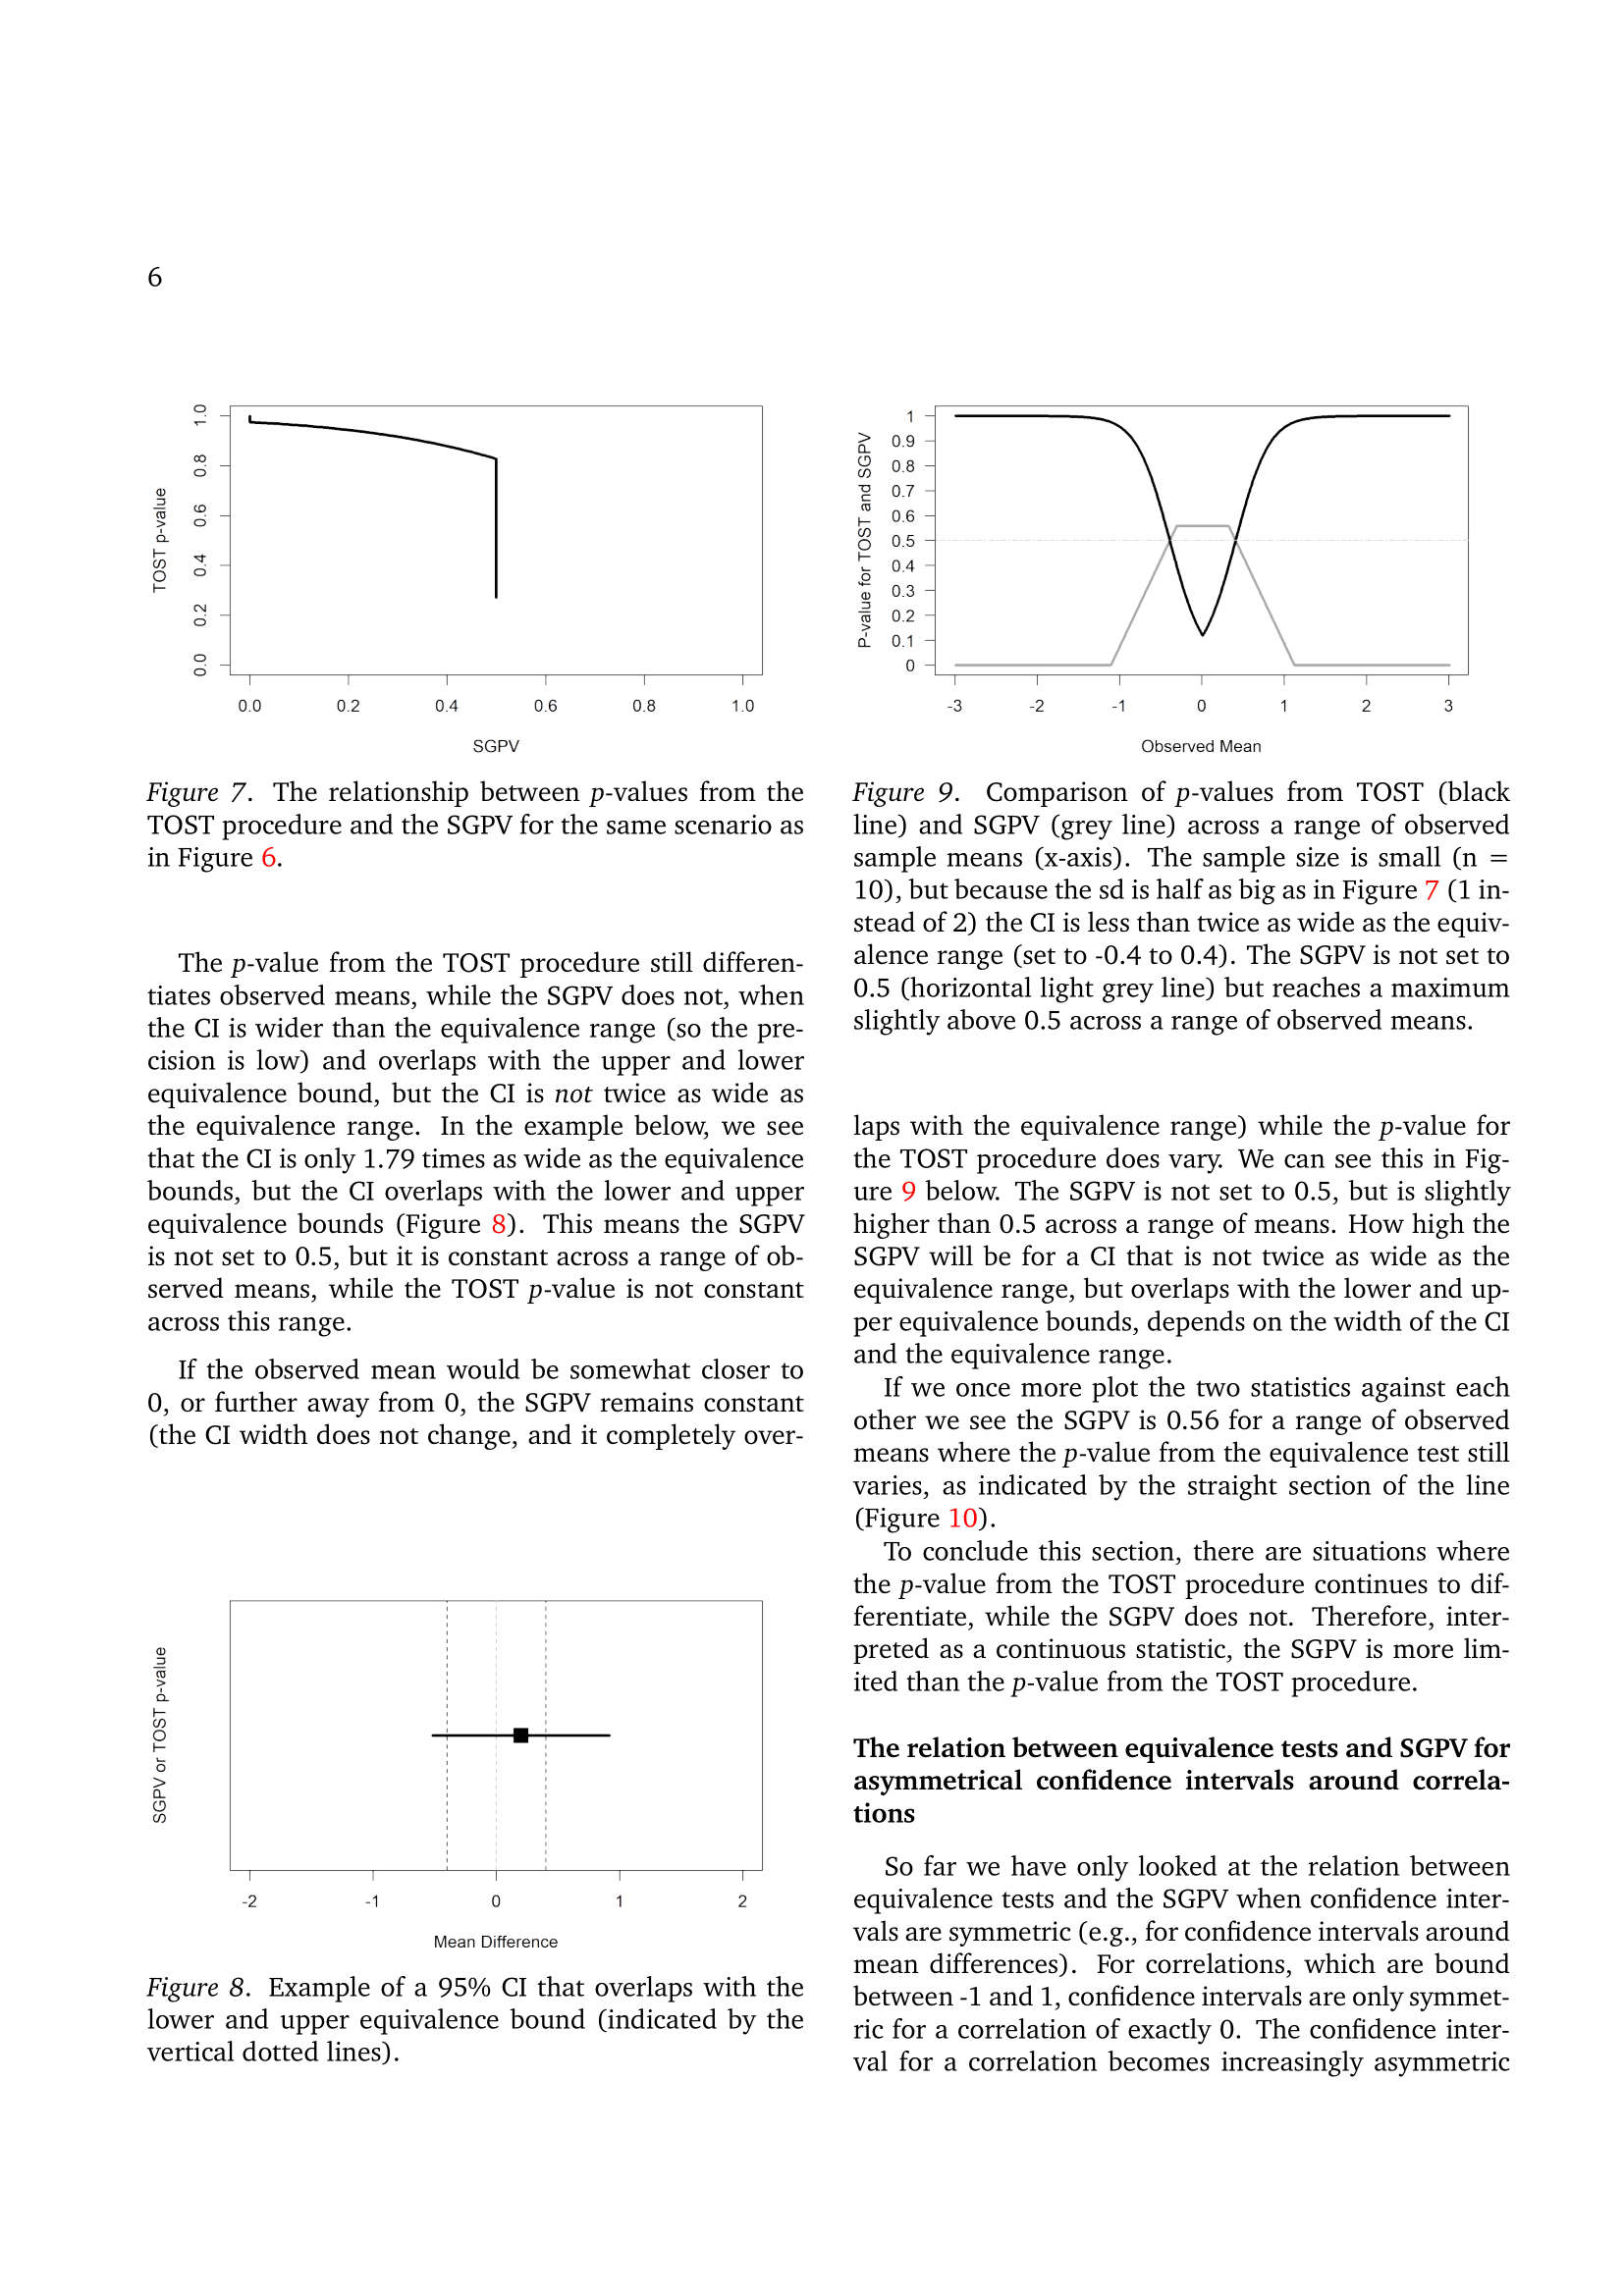
\includegraphics{C:/Users/Admin/Documents/Github projects/thesis/Chapitre 5/Chapitre 5-6} \end{center}

\begin{center}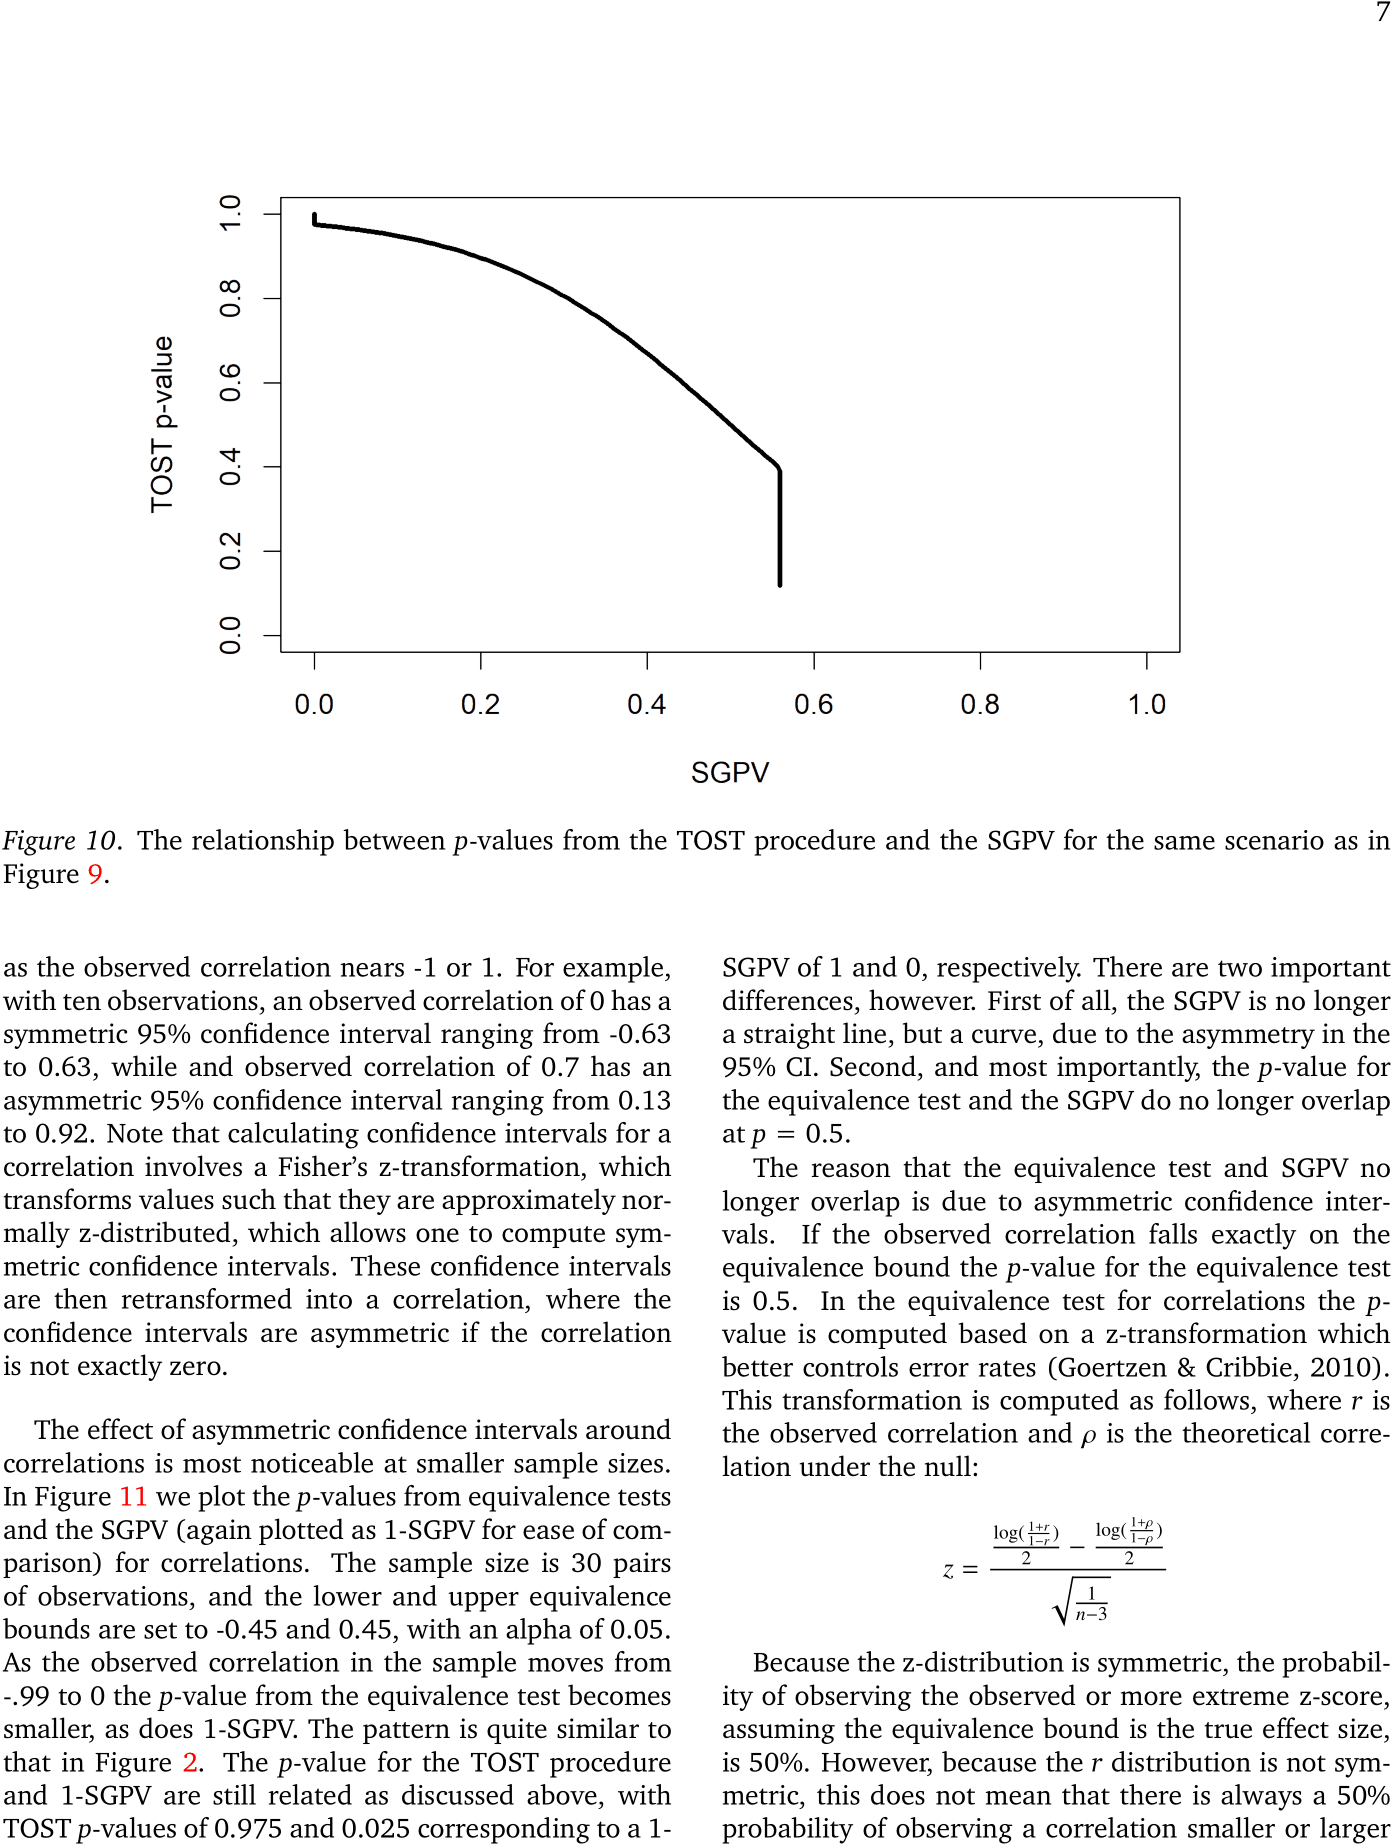
\includegraphics{C:/Users/Admin/Documents/Github projects/thesis/Chapitre 5/Chapitre 5-7} \end{center}

\begin{center}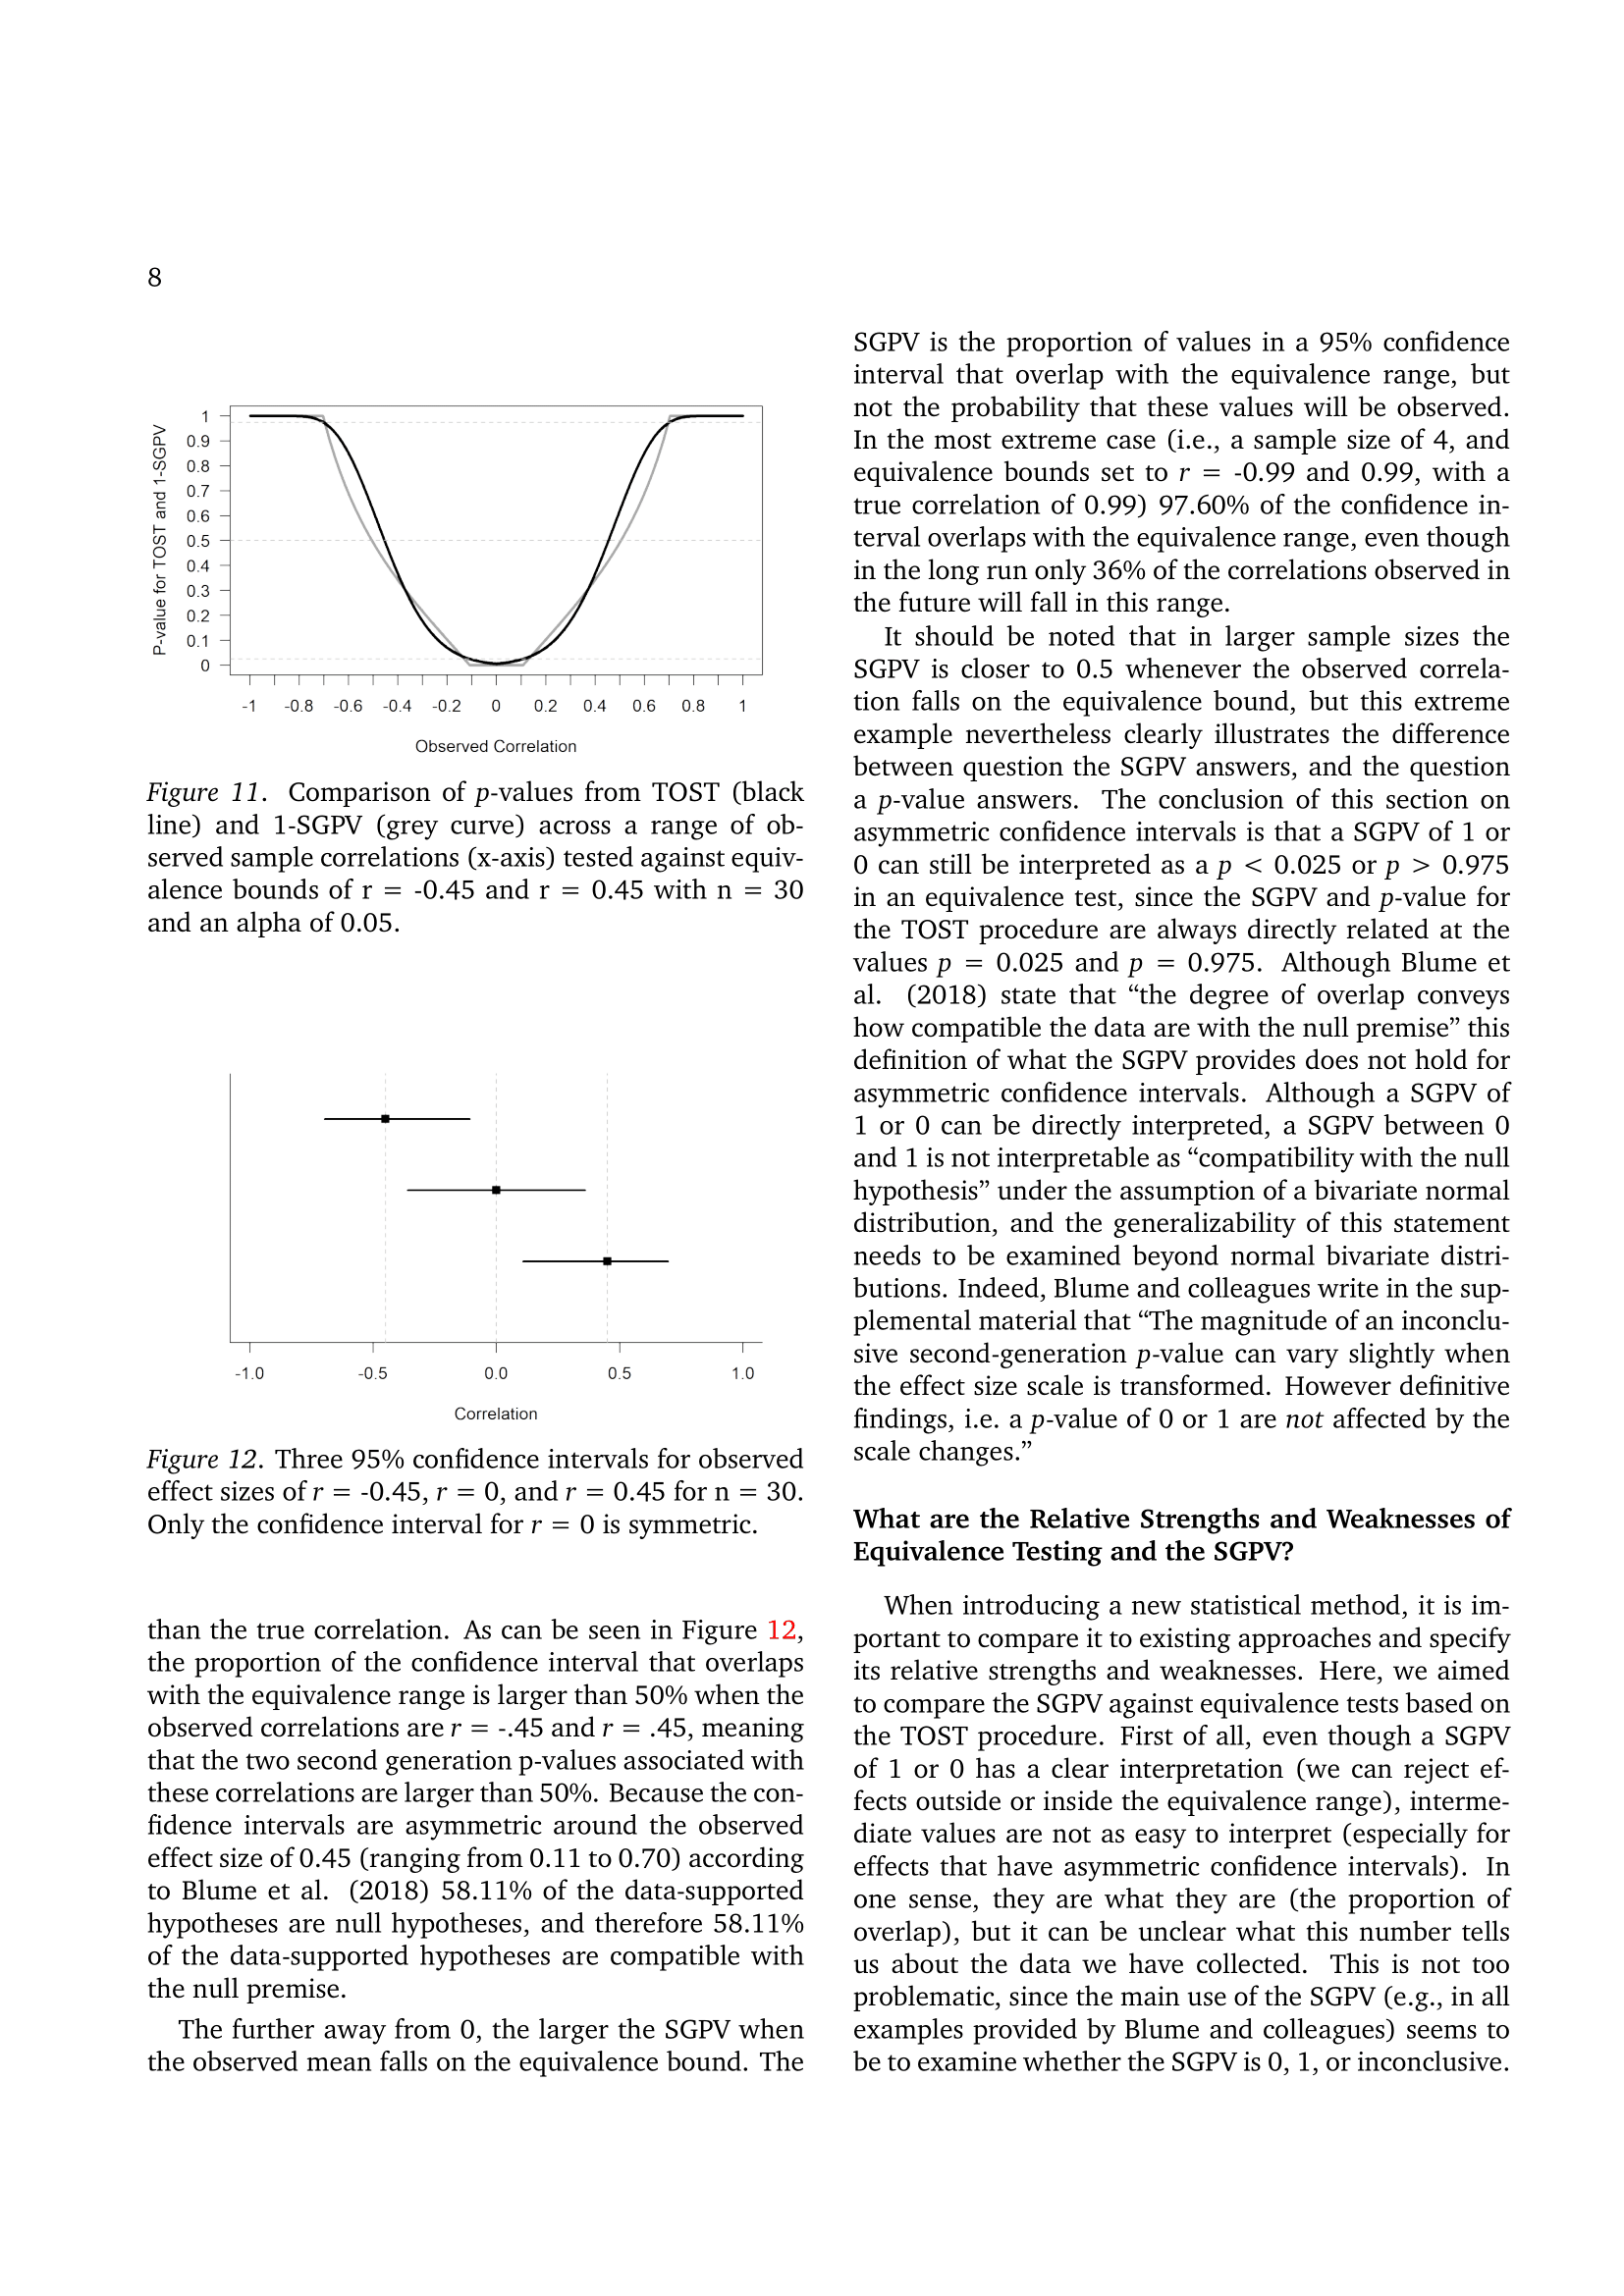
\includegraphics{C:/Users/Admin/Documents/Github projects/thesis/Chapitre 5/Chapitre 5-8} \end{center}

\begin{center}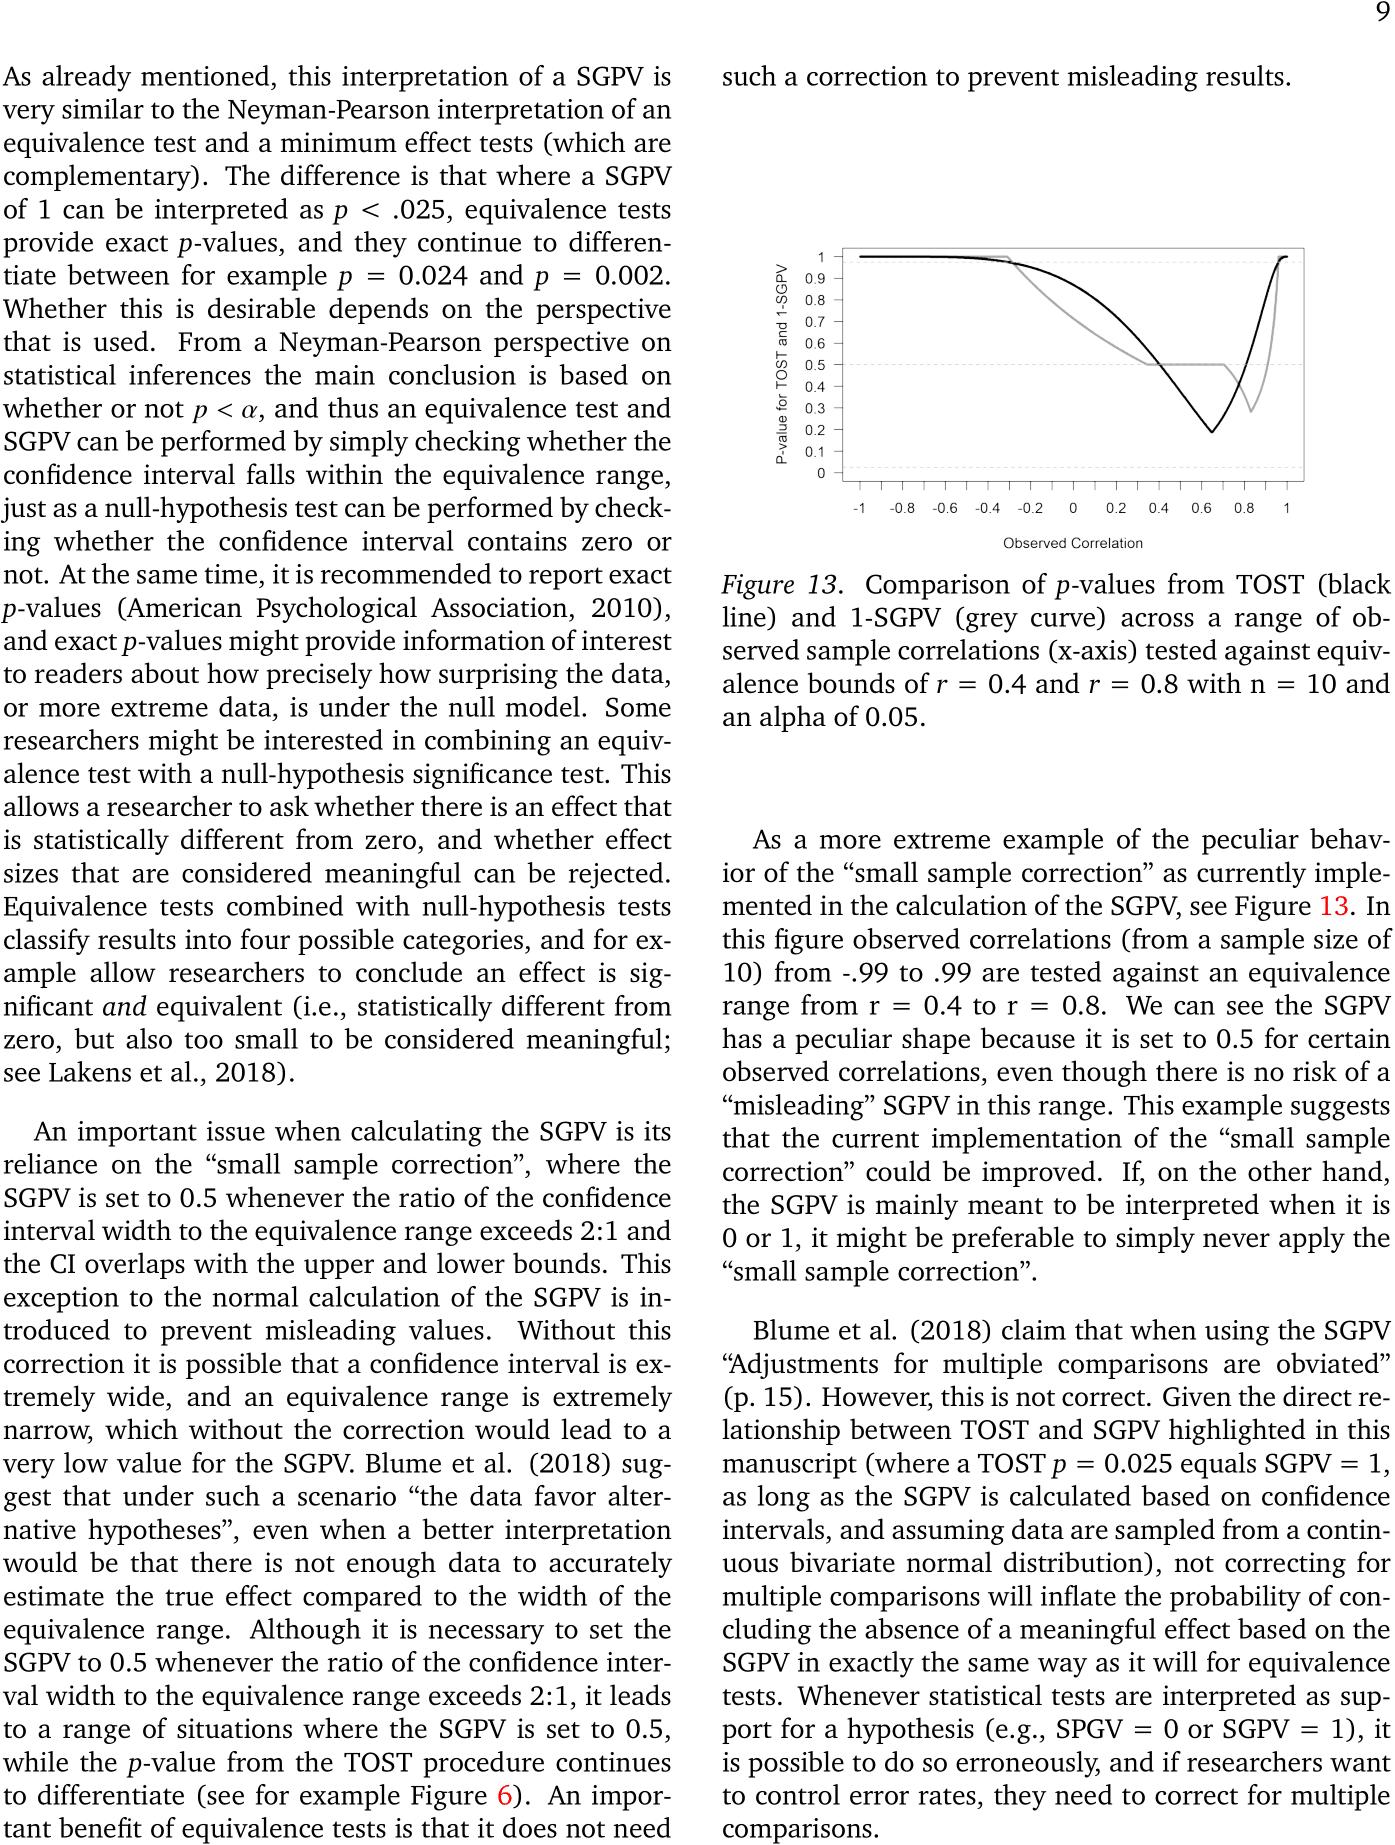
\includegraphics{C:/Users/Admin/Documents/Github projects/thesis/Chapitre 5/Chapitre 5-9} \end{center}

\begin{center}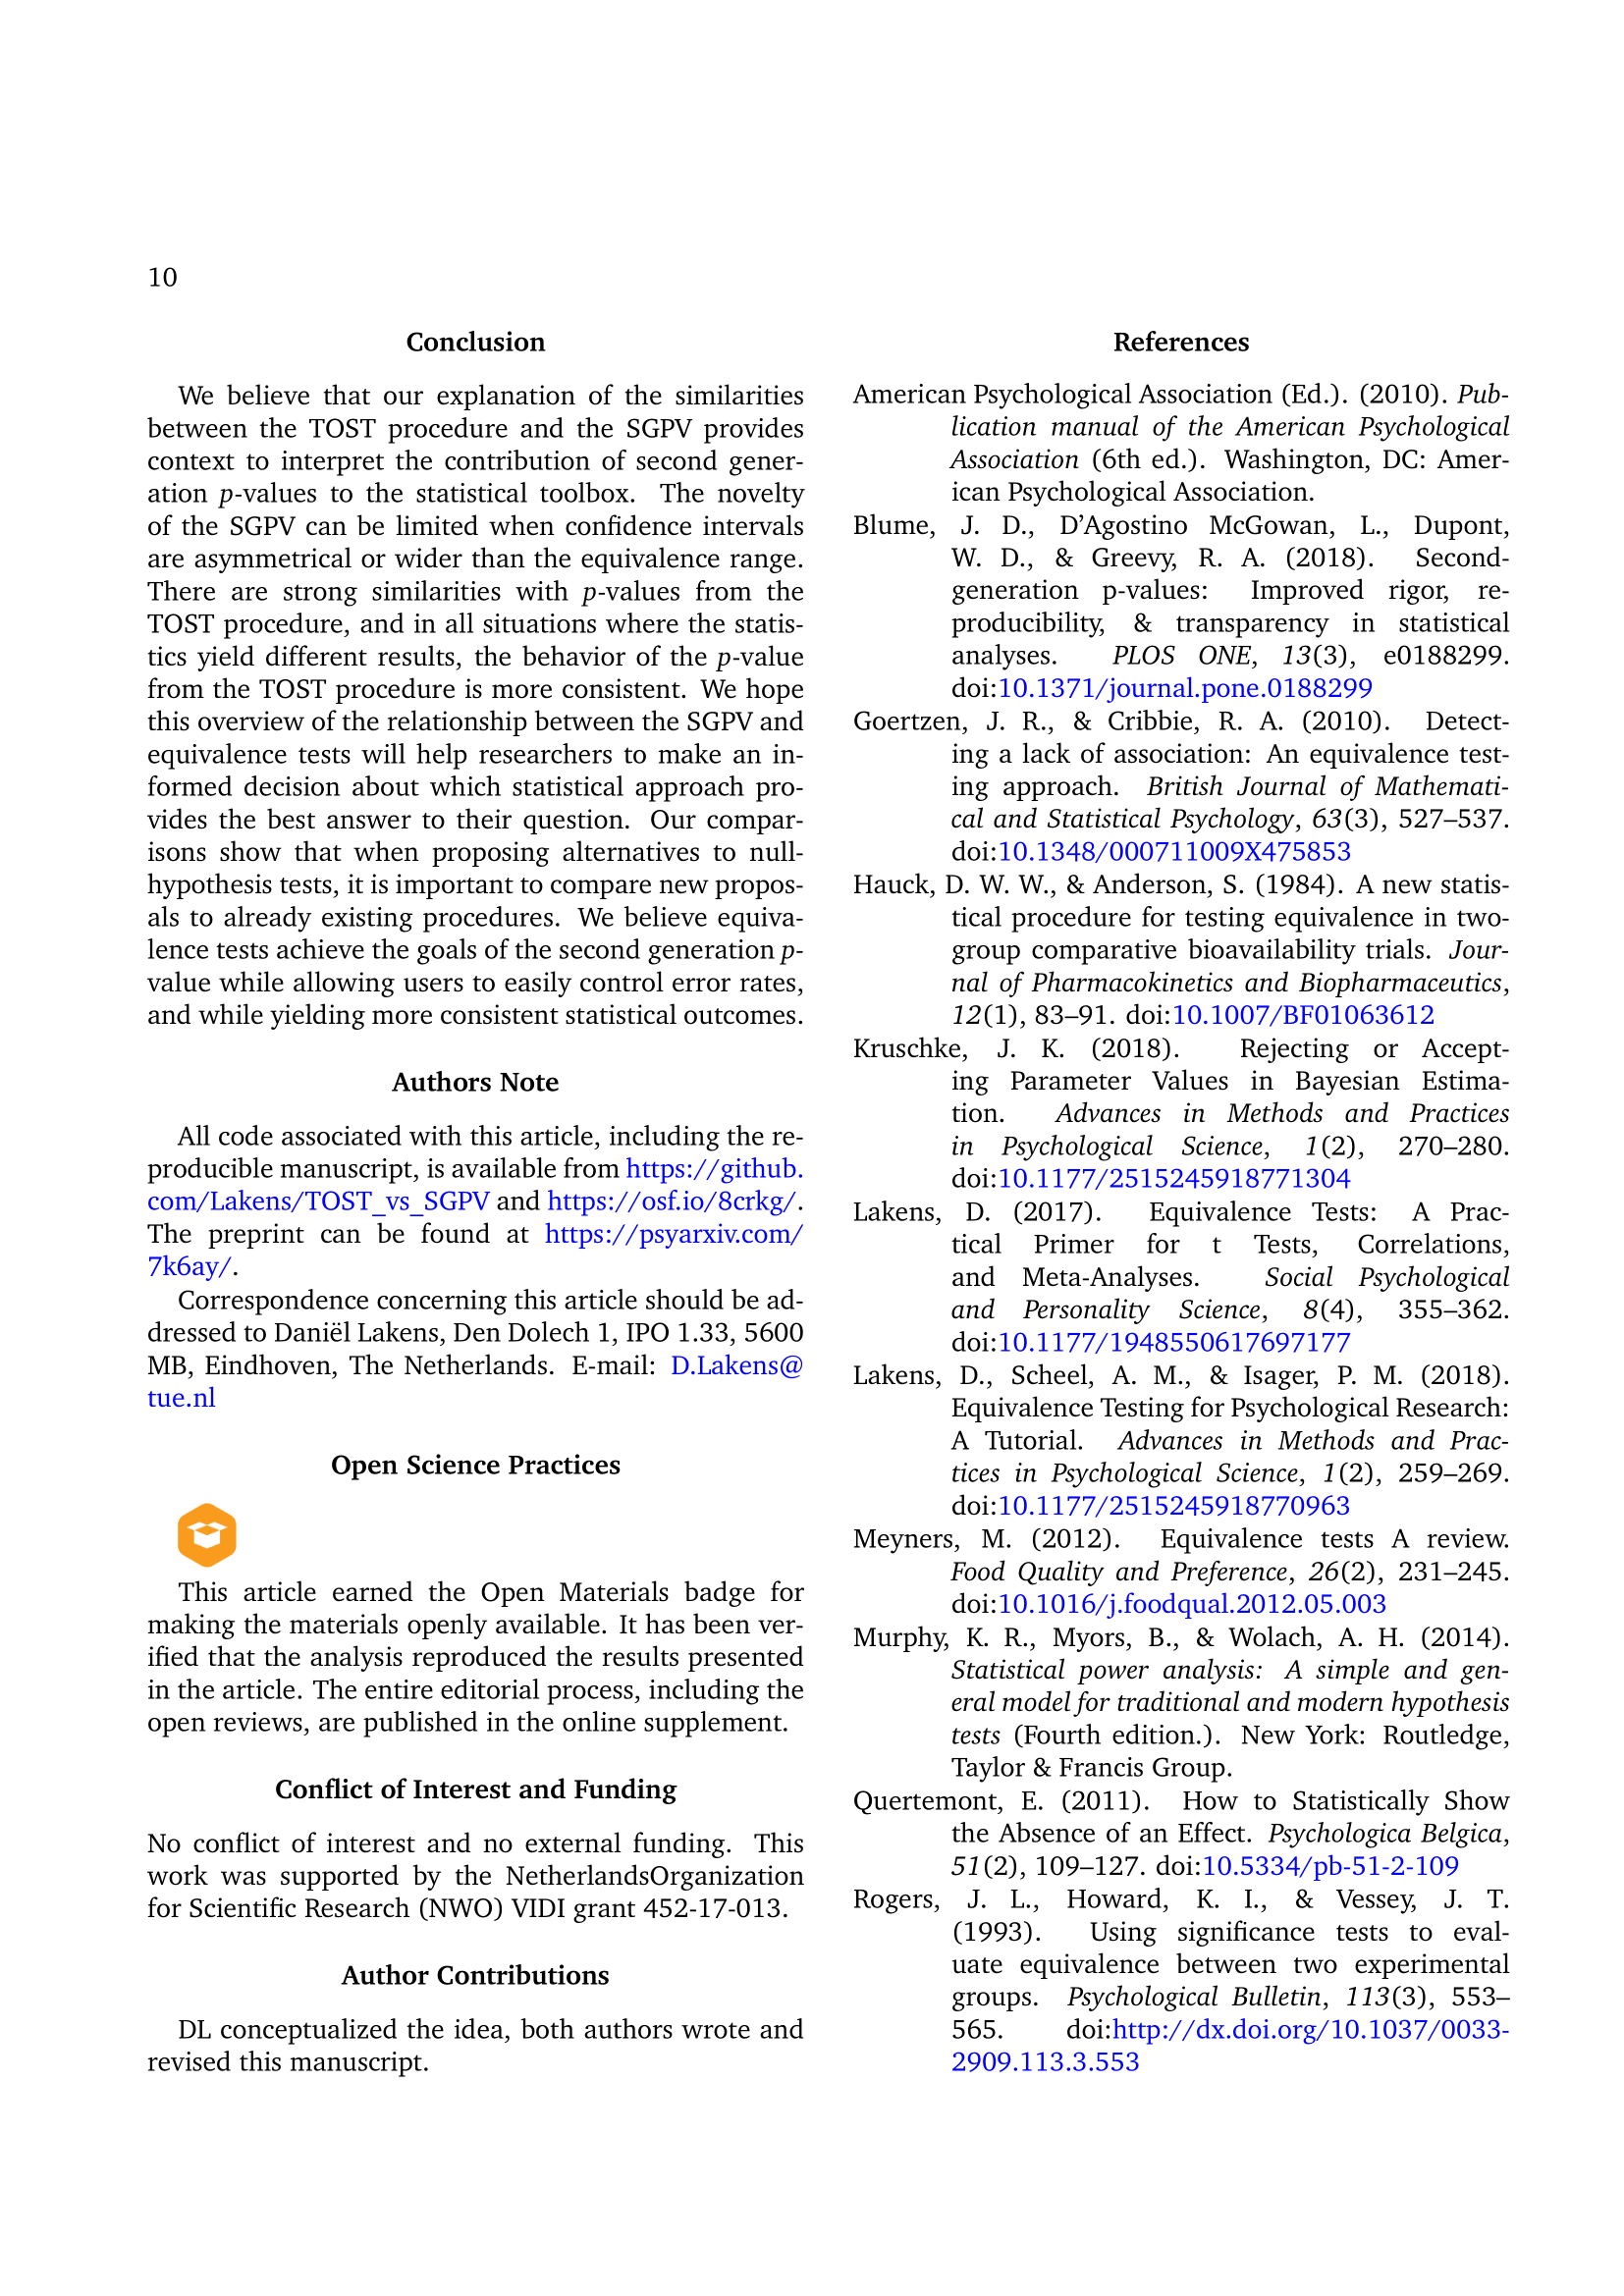
\includegraphics{C:/Users/Admin/Documents/Github projects/thesis/Chapitre 5/Chapitre 5-10} \end{center}

\begin{center}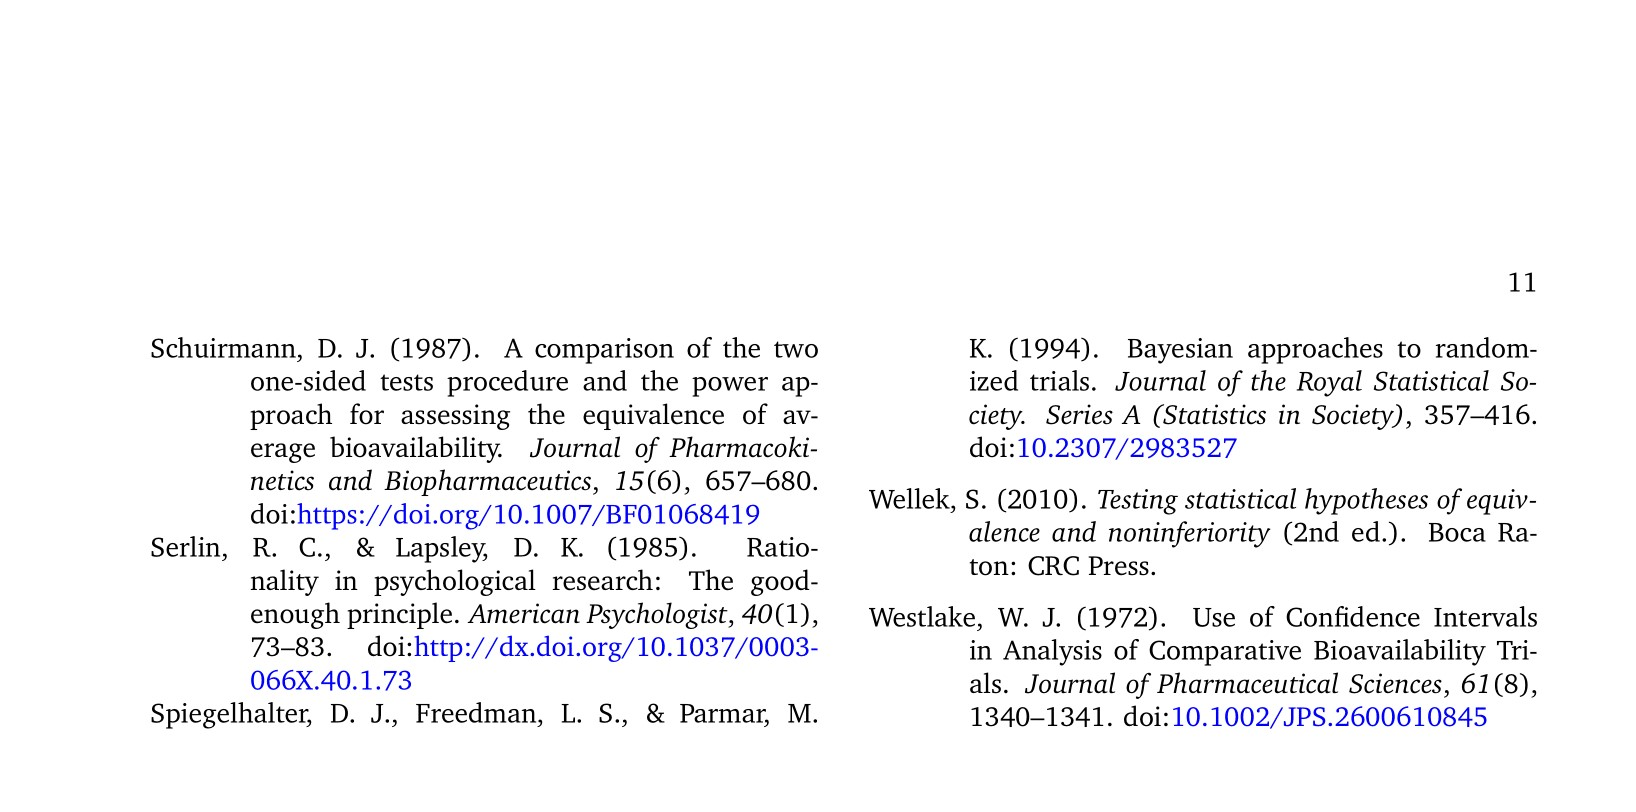
\includegraphics{C:/Users/Admin/Documents/Github projects/thesis/Chapitre 5/Chapitre 5-11} \end{center}


\end{document}
